% This is samplepaper.tex, a sample chapter demonstrating the
% LLNCS macro package for Springer Computer Science proceedings;
% Version 2.20 of 2017/10/04
%
\documentclass[runningheads]{llncs}
%
\usepackage{times}
\usepackage{soul}
\usepackage{url}
\usepackage[hidelinks]{hyperref}
\usepackage[utf8]{inputenc}
%\usepackage[small]{caption}
\usepackage{graphicx}
\usepackage{amsmath}
%\usepackage{amsthm}
\usepackage{booktabs}
%\usepackage{algorithm}
%\usepackage{algorithmic}

\usepackage{enumerate}
\usepackage[linesnumbered,boxed]{algorithm2e}
\usepackage{amstext}
\usepackage{amssymb}
\usepackage{color}
\urlstyle{same}



\usepackage{caption}
\usepackage{subfig}
%\usepackage{subfigure}

% Used for displaying a sample figure. If possible, figure files should
% be included in EPS format.
%
% If you use the hyperref package, please uncomment the following line
% to display URLs in blue roman font according to Springer's eBook style:
% \renewcommand\UrlFont{\color{blue}\rmfamily}

\begin{document}
%
%\title{Forgeting in $\mu$-calculus\thanks{Supported by organization x.}}
\title{On the Weakest Sufficient Conditions in Propositional $\mu$-calculus}
% %
% %\titlerunning{Abbreviated paper title}
% % If the paper title is too long for the running head, you can set
% % an abbreviated paper title here
% %
% \author{First Author\inst{1}\orcidID{0000-1111-2222-3333} \and
% Second Author\inst{2,3}\orcidID{1111-2222-3333-4444} \and
% Third Author\inst{3}\orcidID{2222--3333-4444-5555}}
% %
% \authorrunning{F. Author et al.}
% % First names are abbreviated in the running head.
% % If there are more than two authors, 'et al.' is used.
% %
% \institute{Princeton University, Princeton NJ 08544, USA \and
% Springer Heidelberg, Tiergartenstr. 17, 69121 Heidelberg, Germany
% \email{lncs@springer.com}\\
% \url{http://www.springer.com/gp/computer-science/lncs} \and
% ABC Institute, Rupert-Karls-University Heidelberg, Heidelberg, Germany\\
% \email{\{abc,lncs\}@uni-heidelberg.de}}
% %

\newcommand{\tuple}[1]{{\langle{#1}\rangle}}
%\newcommand{\Dtuple}[2]{{\right\|{#2}\right\|}}
\newcommand{\Mod}{\textit{Mod}}
\newcommand\ie{{\it i.e. }}
\newcommand\eg{{\it e.g.}}
% \newcommand\st{{\it s.t. }}
% \newtheorem{definition}{Definition}
\newtheorem{examp}{Example}
% \newenvironment{example}{\begin{examp}\rm}{\end{examp}}
% \newtheorem{lemma}{Lemma}
% \newtheorem{proposition}{Proposition}
% \newtheorem{theorem}{Theorem}
% \newtheorem{corollary}[theorem]{Corollary}
\iffalse
\newenvironment{proof}{{\bf Proof:}}{\hfill\rule{2mm}{2mm}\\ }
\fi
\newcommand{\rto}{\rightarrow}
\newcommand{\lto}{\leftarrow}
\newcommand{\lrto}{\leftrightarrow}
\newcommand{\Rto}{\Rightarrow}
\newcommand{\Lto}{\Leftarrow}
\newcommand{\LRto}{\Leftrightarrow}
\newcommand{\Var}{\textit{Var}}
\newcommand{\Forget}{\textit{Forget}}
\newcommand{\KForget}{\textit{KForget}}
\newcommand{\TForget}{\textit{TForget}}
\newcommand{\forget}{\textit{forget}}
\newcommand{\Fst}{\textit{Fst}}
\newcommand{\dep}{\textit{dep}}
\newcommand{\term}{\textit{term}}
\newcommand{\literal}{\textit{literal}}

\newcommand{\Atom}{\mathcal{A}}
\newcommand{\SFive}{\textbf{S5}}
\newcommand{\MPK}{\textsc{k}}
\newcommand{\MPB}{\textsc{b}}
\newcommand{\MPT}{\textsc{t}}
\newcommand{\MPA}{\forall}
\newcommand{\MPE}{\exists}

\newcommand{\DNF}{\textit{DNF}}
\newcommand{\CNF}{\textit{CNF}}

\newcommand{\degree}{\textit{degree}}
\newcommand{\sunfold}{\textit{sunfold}}

\newcommand{\Pos}{\textit{Pos}}
\newcommand{\Neg}{\textit{Neg}}
\newcommand\wrt{{\it w.r.t.}}
\newcommand{\Hm} {{\cal M}}
\newcommand{\Hw} {{\cal W}}
\newcommand{\Hr} {{\cal R}}
\newcommand{\Hb} {{\cal B}}
\newcommand{\Ha} {{\cal A}}

\newcommand{\Dsj}{\triangledown}

\newcommand{\wnext}{\widetilde{\bigcirc}}
\newcommand{\nex}{\bigcirc}
\newcommand{\ness}{\square}
\newcommand{\qness}{\boxminus}
\newcommand{\wqnext}{\widetilde{\circleddash}}
\newcommand{\qnext}{\circleddash}
\newcommand{\may}{\lozenge}
\newcommand{\qmay}{\blacklozenge}
\newcommand{\unt} {{\cal U}}
\newcommand{\since} {{\cal S}}
\newcommand{\SNF} {\textit{SNF$_C$}}
\newcommand{\start}{\textbf{start}}
\newcommand{\Elm}{\textit{Elm}}
\newcommand{\simp}{\textbf{simp}}
\newcommand{\nnf}{\textbf{nnf}}

\newcommand{\Diff}{\textrm{Diff}}

\newcommand{\CTL}{\textrm{CTL}}
\newcommand{\Ind}{\textrm{Ind}}
\newcommand{\Tran}{\textrm{Tran}}
\newcommand{\Sub}{\textrm{Sub}}
\newcommand{\NI}{\textrm{NI}}
\newcommand{\Inst}{\textrm{Inst}}
\newcommand{\Com}{\textrm{Com}}
\newcommand{\Rp}{\textrm{Rp}}
%\newcommand{\forget}{{\textsc{f}_\CTL}}
\newcommand{\ALL}{\textsc{a}}
\newcommand{\EXIST}{\textsc{e}}
\newcommand{\NEXT}{\textsc{x}}
\newcommand{\FUTURE}{\textsc{f}}
\newcommand{\UNTIL}{\textsc{u}}
\newcommand{\GLOBAL}{\textsc{g}}
\newcommand{\UNLESS}{\textsc{w}}
\newcommand{\Def}{\textrm{def}}
\newcommand{\IR}{\textrm{IR}}
\newcommand{\Tr}{\textrm{Tr}}
\newcommand{\dis}{\textrm{dis}}
\def\PP{\ensuremath{\textbf{PP}}}
\def\NgP{\ensuremath{\textbf{NP}}}
\def\W{\ensuremath{\textbf{W}}}
\newcommand{\Pre}{\textrm{Pre}}
\newcommand{\Post}{\textrm{Post}}


\newcommand{\CTLsnf}{{\textsc{SNF}_{\textsc{ctl}}^g}}
\newcommand{\ResC}{{\textsc{R}_{\textsc{ctl}}^{\succ, S}}}
\newcommand{\CTLforget}{{\textsc{F}_{\textsc{ctl}}}}
\newcommand{\Muforget}{{\textsc{F}_{\textsc{$\mu$}}}}
\newcommand{\Refine}{\textsc{Refine}}
\newcommand{\cf}{\textrm{cf.}}
\newcommand{\NEXP}{\textmd{\rm NEXP}}
\newcommand{\EXP}{\textmd{\rm EXP}}
\newcommand{\coNEXP}{\textmd{\rm co-NEXP}}
\newcommand{\NP}{\textmd{\rm NP}}
\newcommand{\coNP}{\textmd{\rm co-NP}}
\newcommand{\Pol}{\textmd{\rm P}}
\newcommand{\BH}[1]{\textmd{\rm BH}_{#1}}
\newcommand{\coBH}[1]{\textmd{\rm co-BH}_{#1}}
\newcommand{\Empty}{\emptyset}%\varnothing}
\newcommand{\NLOG}{\textmd{\rm NLOG}}
\newcommand{\DeltaP}[1]{\Delta_{#1}^{p}}
\newcommand{\PIP}[1]{\Pi_{#1}^{p}}
\newcommand{\SigmaP}[1]{\Sigma_{#1}^{p}}


\maketitle              % typeset the header of the contribution
%
\begin{abstract}
The $\mu$-calculus is one of the most important logics describing specifications of transition systems. It has been
extensively explored for formal verification in model checking due to its exceptional balance between expressiveness and algorithmic properties.
On the one hand, some  information content in a specification
might become irrelevant or unnecessary due to various reasons from the perspective of knowledge representation.
On the other hand, a weakest precondition of a specification is badly necessary in verification, where
 a (weakest) precondition is sufficient for a transition system to enjoy a desire property.
 This paper is to address these scenarios for $\mu$-calculus in a principle way in terms of knowledge {\em forgetting}.
In particular, it proposes a
notion of forgetting by a generalized bisimilar equivalence (over a signature) and explores
its important properties as a knowledge distilling operator, besides some reasoning complexity results.
It then shows that how the weakest sufficient condition and the strongest necessary condition can be established
via forgetting. It also discusses knowledge update for $\mu$-calculus in terms of forgetting.

% Propositional $\mu$-calculus is an expressive logic, and also an important specification language in verification.
% One of the common phenomenons in both the verification and the system design is some information content of such specification might become irrelevant for the system due to various reasons e.g., it might be discarded or become obsolete by time, or just become infeasible due to practical difficulties.
% Then, the problem arises on how to distill the information without altering the relevant system behavior or violating the original specification over a given signature.
% Moreover, three crucial notions are vital:  the \emph{strongest necessary condition} (SNC), the \emph{weakest sufficient condition}  (WSC) and the knowledge update.
% To address these scenarios and to target the relevant notions SNC (WSC) and knowledge update in a principled way. In this paper, we explore the knowledge update and SNC (WSC) of $\mu$-calculus from the point of \emph{forgetting}.
% We study its theoretical properties and also show that our notion
% of forgetting satisfies existing essential postulates of knowledge forgetting.
% Furthermore, we show that the reasoning problems of the forgetting are $\textsc{Exptime}$-complete.
\keywords{Weakest precondition \and Forgetting \and Knowledge update.}
\end{abstract}
%
%
%
\section{Introduction}
Propositional $\mu$-calculus is an expressive logic, on binary trees it is as expressive as the monadic second-order logic of two successors (S2S)~\cite{emerson1991tree,niwinski1988fixed}.
%It has been used to verification to specify a needed property.
Subsequent research has shown that the $\mu$-calculus is an important logic when formal specification and verification are concerned.
Let's consider the \emph{model checking} problem, i.e., deciding whether $\Hm \models \varphi$ for a given model $\Hm$ and a specification $\varphi$ (a $\mu$-formula). Currently, most solvers will output ``Yes" if $\Hm$ satisfies $\varphi$, otherwise, they will output ``No" and a counterexample. In this case, a problem is raised on how to compute a \emph{precondition} $\psi$ over a signature such that $\Hm \models \psi \rto \varphi$.
This condition is limited to the weakest one, i.e., the weakest precondition (WP), when addressing ``how to verify a `Hoare triple' $\{\phi\} P\{\psi\}$ where $P$ is a program".
For this reason, E. Dijkstra explored computing the WP for a specification $\psi$ and a given program $P$~\cite{DBLP:journals/cacm/Dijkstra75}.
In this method, it requires the program $P$ will be terminating. 
However, the given model $\Hm$ in model checking problem may be non-terminating, and we cannot use  Dijkstra's method to compute WP.


%Fortunately, it has been shown in~\cite{renyansfirstpaper} that any initial $\MPK$-structure~\footnote{An initial $\MPK$-structure is a pair of Kripke structure $\Hm=(S, r, R, L)$ and its root $r$, i.e. $\tuple{\Hm, r}$, such that: (1) $S$ is finite set of states; (2) $R \subseteq S \times S$ is a total relation; and (3) each sate in $S$ is reachable from $r$.} can be expressed by a \CTL\ formula. In this case, we can use a similar approach, i.e. a forgetting-based approach, to compute WP in $\mu$-calculus.
%Moreover, subsequent research showed that the $\mu$-calculus is an important logic when specification and verification is concerned.
Moreover, whether in verification or system design, a common phenomenon is that some informative content in a specification may be system-independent for a variety of reasons e.g., it may be discarded or become obsolete over time, or it might become unworkable because of practical difficulties.
However, in this case, it is usually expensive and tedious to redesign the specifications meeting the given requirements. An alterative approach is to remove the irrelevant information without changing the behaviour of the associated system or violating the existing system specification for the given signature.

However, it is a non-trivial task~\footnote{Although the model checking for unrestricted \CTL\ can be decided in P (more precisely, even  $O(|S|.|\varphi|)$ [Schnoebelen, P., 2002]), in regard to the forgetting version of the problem, even for the lighter fragment CTL$_{\ALL\FUTURE}$, it is NP-complete  (i.e., $(\Hm,s_0) \models \CTLforget(\varphi, V)$ is \textsc{NP}-complete [Prop. 7 of  Feng et al. 2020]). Hence, one can expect the general problem to be \emph{at least as hard as} \textsc{NP}.
%Even in the lighter fragment CTL$_{\ALL\FUTURE}$, checking whether $\psi \equiv \CTLforget(\varphi, V)$ is $\Sigma_2^p$-complete (Corollary 7.a [Feng et al. 2020], and $\CTLforget(\varphi, V)$ means forgetting the atoms in $V$ from $\varphi$). Hence, one can expect the general problem \emph{at least as hard as} $\Sigma_2^p$.
} to remove some constraints (atoms) from large and complex systems or specifications without affecting working system components or violating the relevant specifications for a given signature.
Moreover, as we have seen that
the strongest post-condition (SP) and the weakest precondition (WP) of a given specification are central to a wide variety of tasks and studies, e.g. in generating counterexamples~\cite{dailler2018instrumenting} and in the refinement of system~\cite{woodcock1990refinement} in verification.
It should be noted that the SP and WP correspond to the \emph{strongest necessary condition} (SNC) and the \emph{weakest sufficient condition}  (WSC), proposed by Lin~\cite{DBLP:Lin:AIJ:2001}, of the specification, respectively.


To address these scenarios and to target the relevant notions of the SNC (WSC) in a principled way
inspired by~\cite{DBLP:Lin:AIJ:2001,renyansfirstpaper}, in this paper, we explore the SNC (WSC) of $\mu$-calculus from the aspect of forgetting.
In particular, we give the definition of forgetting in $\mu$-calculus by using a bisimulation~\cite{browne1988characterizing,Baier:PMC:2008,Yan:AIJ:2009} under infinite models (to distinguish it from computation tree logic (\CTL)~\cite{renyansfirstpaper}). Then, we show whether this notion satisfies the general principles or postulates proposed by Zhang and Zhou~\cite{Yan:AIJ:2009} and the algebraic properties (including modularity, commutativity and homogeneity).
Moreover, we study the relationship between the SNC (WSC) and forgetting.


Forgetting in propositional logic (PL) and knowledge forgetting in S5 modal logic have been defined and used in the field of \emph{belief update/revision} and \emph{knowledge update}, respectively\cite{DBLP:journals/ai/Lin01,lang2003propositional,su2004reasoning,baral2005knowledge,Zhang2009Knowledge}.
Intuitively, if $\varphi$ represents the agent's belief about the world and the agent performs an action that is supposed to make $\psi$ true in the resulting world, then the agent's belief about the resulting  world can be described by $\varphi \diamond \psi$, where $\diamond$ is the selected update operator.
We can see that the theory of belief updates does not tell us how to perform updates with  respect to this gain in knowledge due to a sensing action.
In this sense, analogous to the notion of belief update, the \emph{knowledge update} was proposed by Baral and Zhang in~\cite{baral2005knowledge} to solve the belief updates caused by sensing actions, in which the effect of a sensing action is expressed by introducing the modal operator (K)nows.
And then knowledge update was defined by forgetting in S5 modal logic~\cite{Zhang2009Knowledge}.
%Nevertheless, there is no approach to solve the knowledge update in logic languages that contain \emph{temporal operators}.


After exploring the definition and properties of forgetting in $\mu$-calculus, we demonstrate how forgetting can be used in knowledge update in $\mu$-calculus in this paper.
In addition, we also show that our definition of knowledge update operator $\diamond_{\mu}$ by forgetting satisfies the update postulates of  Katsuno and Mendelzon~\cite{katsuno91mendelzon}.
%It is worth noting that we require the models to be finite in the knowledge update part in order to express each model with a formula.

The rest of the paper is organized as follows. 
After discussing the related work in the next section, the basic notation and technical preliminaries are introduced in Section~\ref{preliminaries}. The formal definition of forgetting in $\mu$-calculus,  its various properties and the computational complexities are presented in Section~\ref{forgetting}.
Section~\ref{applications} shows the forgetting can be used to comupte both WSC (SNC) and knowledge update.
%Section~\ref{ns_conditions} identifies the WSC by forgetting.
%Section~\ref{knowledge_updat} addresses the knowledge update of $\mu$-calculus by forgetting.
Finally, concluding remarks are given in Section~\ref{sec:conclude}.

To avoid hindering the flow of content, detailed proofs of the technical results are provided in the Appendix.

\section{Related work}
In this section, we briefly discuss published matter that is technically related to our work.

\subsection{The Weakest Precondition}
%hoare triple, WP, invariant, ÏêϸÃèÊöѽ
%Recall that in formal verification,


The \emph{weakest precondition}, as an important concept in formal verification, was first proposed %~\cite{Dijkstra:1959}
by Dijkstra to solve the problem of computing or approximating invariants appearing in the  \emph{verification of computer programs and systems}~\cite{DBLP:journals/cacm/Dijkstra75}, particularly in the ``Hoare triple"~\cite{Hoare1969}.
Afterwards, it was wildly studied in various fields, especially in generating counterexamples~\cite{dailler2018instrumenting} and refining system~\cite{woodcock1990refinement}.

In the field of AI, there is a similar concept called the \emph{weakest sufficient condition} (WSC), which was introduced by Lin to generate successor state axioms from causal theories~\cite{DBLP:Lin:AIJ:2001}. Moreover, the SNC and WSC for proposition $q$ on a restricted subset of the propositional variables under propositional theory $T$ are computed based on the notion of forgetting.
Afterwards the SNC and WSC were generalized to first-order logic (FOL) and a direct method based
on the \emph{second-order quantifier elimination} (SOQE) technique was proposed to automatically generate the SNC and WSC~\cite{doherty2001computing}. In addition, a forgetting-based method is used to compute the SNC and WSC in \CTL~\cite{renyansfirstpaper}.

\subsection{Forgetting}
\emph{Forgetting}
%,
%which is a dual concept of {\em uniform interpolation}~\cite{visser1996uniform,konev2009forgetting}, 
was first formally defined in PL and FOL by Lin and Reiter~\cite{lin1994forget,eiter2019brief}.
As a technique for distilling knowledge, it has been explored in various of logic languages and widely used in AI. % (see the survey \cite{eiter2019brief} for more detail).
Except for the WSC (SNC), belief update/revision, and knowledge update talked about in the Introduction, forgetting has been used for conflict solving~\cite{DBLP:Zhang:AIJ2006,Lang2010Reasoning} and knowledge compilation~\cite{Bienvenu2010Knowledge}.
Informally, forgetting is used to abstract from a knowledge base ${\cal T}$ only the part that is relevant to a subset of alphabet ${\cal P}$ while not affecting the results of ${\cal T}$ on ${\cal P}$.

The concept of forgetting can be traced back to the work of Boole on \emph{propositional
	variable elimination} and the seminal work of Ackermann~\cite{ackermann1935untersuchungen}, who recognised that the problem amounts to \emph{the elimination of existential second-order quantifiers}.
Moreover, it has been extended  to various logic systems, including modal logics~\cite{Yan:AIJ:2009,fang2019forgetting} and nonmonotonic logics~\cite{DBLP:journals/jair/WangZZZ14,gonccalves2020limits}.


%Usually, the definition of forgetting can be defined from the perspective of \emph{strong (or semantic) forgetting} and \emph{weak forgetting}~\cite{Zhang:KR:2010}.
%We consider semantic forgetting (abbreviated to forgetting) and give its definition in CPL and FOL here.

In PL, forgetting has often been studied under the name `variable
elimination'. Formally, the solution of forgetting a propositional variable $p$ from a PL formula $\varphi$ is $\varphi[p/\bot] \vee \varphi[p/\top]$~\cite{lin1994forget}, where $\varphi[p/\bot]$ and $\varphi[p/\top]$ denote the formulas obtained from $\varphi$ by replacing atom $p$ with $\bot$ and $\top$, respectively.


In FOL, the definition of forgetting was defined from the perspective of \emph{strong (or semantic) forgetting} and \emph{weak forgetting}~\cite{Zhang:KR:2010}.
Although  weak forgetting and strong forgetting are not exactly the same, they coincide when the result of strong forgetting exists.
We consider semantic forgetting (abbreviated to forgetting) and give its definition in PL and FOL here.
Forgetting is considered an instance of the SOQE problem in FOL. In that case, the result of forgetting an n-ary predicate $P$ from a first-order formula $\varphi$ is $\exists R \varphi[P/R]$~\cite{lin1994forget}, in which $R$ is an n-ary predicate variable and $\varphi[X/Y]$ is a result of replacing every occurrence of $X$ in $\varphi$ by $Y$. The task of forgetting in FOL, as a computational problem, is to find a first-order formula that is equivalent to $\exists R \varphi[P/R]$. It is evident that this is an SOQE problem. However, the solution to the SOQE problem is not always expressible in FOL~\cite{gabbay2008second},which means that the results of forgetting in FOL are not always expressible in FOL, i.e., forgetting in FOL is \emph{not closed}.
Nonetheless, the solution of weak forgetting is always expressible in FOL, although
there are cases in which the forgetting solution can be represented only by an infinite set of
FOL formulas~\cite{Zhang:KR:2010}. %~\cite{zhang2010forgetting}.
See~\cite{eiter2019brief} for a recent and comprehensive survey.

In non-classical logics,
%in~\cite{Yan:AIJ:2009},
the knowledge forgetting of S5 modal logic was defined~\cite{Yan:AIJ:2009}.
In this paper, the authors shown that the knwoledge update can be represented through knowledge forgetting.
% and explored to show the relationship between knowledge forgetting and knowledge update~\cite{Yan:AIJ:2009}. 
 In addition, they proposed four general postulates for knowledge forgetting and showed that these four postulates precisely characterize the notion of knowledge forgetting in S5 modal logic.
Moreover, they show that \emph{uniform interpolation} ~\cite{visser1996uniform} is a dual concept of forgetting in S5 and PL. 
 These notions were recently extended to multi-agent modal logics~\cite{fang2019forgetting} and CTL~\cite{feng2020sufficient}.
Furthermore, in the scenario of non-monotonic reasoning,  forgetting in logic programs under answer set semantics has been extensively investigated from the perspective of various forgetting postulates~\cite{DBLP:Zhang:AIJ2006,DBLP:journals/ai/EiterW08,Wong:PhD:Thesis,Yisong:JAIR,Yisong:IJCAI:2013,DBLP:journals/jair/Delgrande17,gonccalves2020limits}, see~\cite{eiter2019brief,gonccalves2021forgetting} for a comprehensive survey.
Similarly, the forgetting in description logics (DL) are also explored with the motivation of constructing restricted ontologies by eliminating concept and role symbols from DL-based
ontologies~\cite{Wang:AMAI:2010,Lutz:IJCAI:2011,Konev:JAIR:2012,Zhao:2017:IJCAI,DBLP:conf/aaai/ZhaoSWZF20}. 

It should be mentioned that the existing forgetting definitions in PL and answer set programming are not directly applicable in modal logics.
We cannot directly use the method of forgetting in $\CTL$~\cite{renyansfirstpaper} since it will not work when the  models of the formula are infinite.
Hopefully, it has been proved that the modal $\mu$-calculus has \emph{uniform interpolation}~\cite{d1996uniform}. Informally, for every $\mu$-sentence $\varphi$ and every finite set $V$ of atoms, there exists a $\mu$-sentence $\widetilde{\exists}V \varphi$ that does not contain atoms from $V$ but is  logically closest to $\varphi$ in some sense. 
As we will show that our forgetting definition is equivalent to the semantic definition of uniform interpolation in~\cite{d1996uniform,d2006modal}.
%This means that the result of forgetting some atoms from a $\mu$-calculus sentence always exists. 
In the sense, showing the semantics of forgetting in $\mu$-calculus through \emph{general principles or postulates} is important to make it easier to understand.

\section{Preliminaries}  \label{preliminaries}
In this section, we introduce the technical and notational preliminaries, i.e., the  syntax and semantics of $\mu$-calculus, closely related to this paper.
Moreover, throughout this paper, we denote by $\overline V$ the complement of $V \subseteq B$ on a given set $B$, i.e., $\overline V = B -V$.

\subsection{The syntax of $\mu$-calculus}\label{mu-suntax}
Modal $\mu$-calculus is an extension of modal logic, and we consider the propositional $\mu$-calculus introduced by Kozen~\cite{DBLP:journals/cacm/Kozen83}.
Let $\Ha=\{p,q,\dots\}$ be a set of propositional letters (atoms) and ${\cal V}=\{X, Y, \dots\}$ be a set of variables.
Then, the formulas of the $\mu$-calculus, called $\mu$-formulas (or formulas), over these sets can be inductively defined in Backus-Naur form:
\[
\varphi := p\ |\ \neg p\ |\ X\ |\ \varphi \vee \varphi\ |\ \varphi \wedge \varphi \ |\ \EXIST\NEXT \varphi\ |\ \ALL\NEXT \varphi\ |\ \mu X. \varphi\ |\ \nu X. \varphi
\]
where $p\in \Ha$ and $X\in {\cal V}$. $\top$ and $\bot$ are also $\mu$-calculus formulas, which express `true' and `false', respectively.
The variable $X$ is said to be bound in $\mu X. \varphi$, $\nu X. \varphi$.
%Besides, $X$ occurs just positively in $\varphi$ (that is to say $X$ appears after an even number of negations).

It is obvious that negations, i.e., `$\neg$', are allowed only before propositional letters.
%Note that we allow negations only before propositional letters.
All the results
presented here extend to the general case where negation before variables is also
allowed, restricted as usual to positive occurrences of bound variables; that is variables appear after an even number of negations.
Variables, propositional letters and their negations are called \emph{literals}.
For convenience, in the following, $\varphi$, $\varphi_1$, \dots, $\psi$, $\psi_1$, \dots\ are used to denote $\mu$-formulas.
By $\Var(\varphi)$ we mean the set of atoms appearing in formula $\varphi$.



A formula is \emph{well\ named} iff every variable is bound at most once in the formula, and free variables are distinct from bound
variables. For a variable $X$ bound in a well named formula $\varphi$ there exists a unique subformula of $\varphi$ of the form $\delta X. \psi(X)$ with $\delta \in \{\nu, \mu\}$.
%, from now on called the \emph{binding definition}
%of $X$ in $\varphi$. We call $X$ a $\mu$-variable when $\delta = \mu$, otherwise we call $X$ a $\nu$-variable.

Variable X in $\delta X. \varphi(X)$ is \emph{guarded} iff every occurrence of $X$ in
$\varphi(X)$ is within the scope of some modality operators $\EXIST \NEXT$ or $\ALL \NEXT$.
A formula is guarded iff every bound variable in the formula is guarded. Furthermore, a \emph{$\mu$-sentence} is a formula containing no free
variables.%, i.e., no variables unbound by an operator.

In the following, we restrict ourselves to \textbf{guarded}, \textbf{well-named} $\mu$-sentences.


\subsection{The semantics of $\mu$-calculus}\label{mu-semantic}
%We are now in the position to recall the semantics of $\mu$-formulas.
Generally, $\mu$-formulas are interpreted in transition systems of the form $\Hm = (S, r, R, L)$, which we call a Kripke structure, where:
\begin{itemize}
	\item $S$ is a nonempty set of states,
	\item $r\in S$,
	\item $R$ is a binary relation on $S$, i.e. $R \subseteq S \times S$, called a transition relation, and
	\item $L: S \rto 2^{\Ha}$ is a labeling function.
\end{itemize}
Sometimes, $r$ is called the `\emph{root}' of $\Hm$~\cite{d2000logical}. A Kripke structure $\Hm$ is finite if $S$ is finite and 
for each state $s\in S$, there is $q \not \in L(s)$ for almost all $q\in \Ha$.
%$q \not \in L(s)$ (for each state $s\in S$) for  almost all $q\in \Ha$.

Given a Kripke structure $\Hm$ and a valuation $v: {\cal V} \rto 2^S$, the set of states
in which a formula $\varphi$ is true, denoted as $\left\| \varphi\right\|_v^{\Hm}$, is defined inductively as follows (the superscript $\Hm$ is omitted when doing so causes no ambiguity):
%(we will omit superscript $\Hm$ when it causes no ambiguity):
\begin{align*}
	& \left \| p\right \|_v = \{s\ |\ p \in L(s)\} \ ;\ \left\|\top\right\|_v = S \ ;\ \left\|\bot\right\|_v = \emptyset; \\
	& \left\|\neg p\right\|_v = S- \left\| p\right\|_v;\\
	& \left\| X\right\|_v = v(X);\\
	& \left\|\varphi_1 \vee \varphi_2\right\|_v = \left\|\varphi_1\right\|_v \cup \left\|\varphi_2\right\|_v;\\
	& \left\|\varphi_1 \wedge \varphi_2\right\|_v = \left\|\varphi_1\right\|_v \cap \left\|\varphi_2\right\|_v;\\
	& \left\|\EXIST \NEXT \varphi\right\|_v = \{s| \exists s'. (s, s') \in R \wedge s' \in \left\|\varphi\right\|_v\};\\
	& \left\|\ALL \NEXT \varphi\right\|_v = \{s| \forall s'. (s, s') \in R \Rto s' \in \left\|\varphi\right\|_v\};\\
	& \left\| \mu X. \varphi\right\|_v = \bigcap\{S' \subseteq S | \left\|\varphi\right\|_{v[X:= S']} \subseteq S'\};\\
	& \left\| \nu X. \varphi\right\|_v = \bigcup\{S' \subseteq S | S' \subseteq \left\|\varphi\right\|_{v[X:= S']}\}.
\end{align*}
where $v[X:= S']$ is the same as the valuation function $v$ except that $S'$ is assigned to $X$, i.e., for each $Y\in {\cal V}$:
\[v[X:= S'](Y) =
\left\{
\begin{array}{ll}
	S', \ \ \qquad \qquad \qquad \hbox{if $Y = X$;} \\
	v(Y), \ \ \ \qquad \qquad \ \ \hbox{otherwise.}
\end{array}
\right.
\]

In the following, we denote $s\in \left\| \varphi \right\|_v$ by $(\Hm, s, v) \models \varphi$ and we may leave out the
valuation $v$ if $\varphi$ is a $\mu$-sentence.
$(\Hm, v) \models \varphi$ is used to denote $(\Hm, r, v) \models \varphi$.
$(\Hm,v)$ is a \emph{model} of $\varphi$ whenever  $(\Hm, v) \models \varphi$.
In this case, $\Mod(\varphi)$ denotes the set of models of $\varphi$.
Particularly, if $\varphi$ is a $\mu$-sentence, then we use $\Hm \models \varphi$ to replace $(\Hm, v) \models \varphi$ and $\Mod(\varphi) = \{\Hm \mid \Hm \models \varphi\}$.
Similarly, let $\Sigma$ be a set of $\mu$-sentences; we define $\Mod(\Sigma)$ as the set of Kripke structures $\Hm$ such that $\Hm \models \varphi$ for each $\varphi\in \Sigma$.
Moreover, $\psi$ is a \emph{logical consequence} of $\varphi$, denoted by $\varphi \models \psi$, if $(\Hm,v ) \models \varphi$ then $(\Hm,v) \models \psi$ for every Kripke structure $\Hm$ and valuation $v$.
%$\varphi \models \psi$ denotes \emph{logical consequence}: if $(\Hm,v ) \models \varphi$ then $(\Hm,v) \models \psi$ for every Kripke structure
%$\Hm$ and valuation $v$.
Particularly, given two sentences (or set of sentences) $\Sigma$ and $\Pi$, $\Sigma \models \Pi$ if $\Mod(\Sigma) \subseteq \Mod(\Pi)$. And $\Sigma \equiv \Pi$ whenever $\Mod(\Sigma) = \Mod(\Pi)$; in this case we also call $\Sigma$ and $\Pi$ \emph{semantically  equivalent}.

A $\mu$-sentence $\phi$ is {\em irrelevant to} the atoms in a set $V$ (or simply $V$-{\em irrelevant}), written $\IR(\phi,V)$,
if there is a $\mu$-sentence $\psi$ with $\Var(\psi)\cap V=\emptyset$ such that $\phi\equiv\psi$.
The $V$-{\em irrelevance} of a set of $\mu$-sentences can be defined similarly, i.e., a set $\Sigma$ of $\mu$-sentences is irrelevant to the atoms in $V$, written $\IR(\Sigma, V)$, if $\IR(\varphi, V)$ for each $\varphi \in \Sigma$.


\subsection{Disjunctive $\mu$-formula}
The disjunctive formula of $\mu$-formula originate from the work in~\cite{janin1995automata}.
In this paper, we use the definition of disjunctive $\mu$-formula in~\cite{d2006modal}.

An alternative syntax for the $\mu$-calculus, called \emph{covers-syntax}, is obtained by substituting the $\EXIST\NEXT$ operator with a set of \emph{cover operators}, one for each natural $n$.
In this way, $Cover(\emptyset)$ is a $\mu$-formula and for $n \geq 1$, if $\varphi_1, \dots, \varphi_n$ are formulas, then
\[
Cover(\varphi_1, \dots, \varphi_n)
\]
is a formula. For a given Kripke structure $\Hm = (S,r,R,L)$, $Cover(\emptyset)$ is true in $\Hm$ if and only if the root of $\Hm$ does not have any successor, while $Cover(\varphi_1, \dots, \varphi_n)$ is true in $\Hm$ if and only if the successors
of the root are covered by $\varphi_1, \dots, \varphi_n$. More formally, $(\Hm, s,v ) \models Cover(\varphi_1, \dots, \varphi_n)$ with $s \in S$
if and only if:
\begin{itemize}
	\item for every $i = 1, . . . , n$, there exists $t$ with $(s, t) \in R$ and $(\Hm, t,v) \models \varphi_i$;
	\item for every $t$ with $(s, t) \in R$ there exists $i\in \{1, . . . , n\}$ with $(\Hm, t,v) \models \varphi_i$.
\end{itemize}

It has shown that the $\mu$-calculus obtained from the covers-syntax is equivalent to the familiar $\mu$-calculus talked in subsection~\ref{mu-suntax}\cite{d2006modal}.

%Although they are the same in the semantics, we use the definition of the disjunctive formula in G in this paper.
%  We now introduce an important class of $\mu$-formulas, i.e., the \emph{disjunctive formula}.
\begin{definition}[disjunctive $\mu$-formula~\cite{d2006modal}]
	The set of disjunctive $\mu$-formulas, ${\cal F}_d$ is the smallest set containing $\top$, $\bot$, and non-contradictory conjunciton of literals which is closed under:
	\begin{itemize}
		\item[(1)] disjunctions: if $\alpha, \beta \in {\cal F}_d$, then $\alpha \vee \beta \in {\cal F}_d$;
		\item[(2)] special conjunctions: if $\varphi_1, \dots, \varphi_n\in {\cal F}_d$ and $\delta$ is a non-contradictory
		conjunction of literals, then $\delta \wedge Cover(\varphi_1, \dots, \varphi_n) \in {\cal F}_d$;
		\item[(3)] fixpoint operators: if $\varphi\in  {\cal F}_d$, $\varphi$ does not contain $X \wedge \psi$ as a subformula for
		any formula $\psi$, and $X$ is positive in $\varphi$, then $\mu X. \varphi$ and $\nu X. \varphi$ are in ${\cal F}_d$.
	\end{itemize}
	
\end{definition}
%\begin{definition}[disjunctive formula~\cite{janin1995automata}]
%	The set of disjunctive formulas, ${\cal F}_d$ is the smallest set defined by the following clauses:
%	\begin{itemize}
%		\item[(1)] every variable is a disjunctive formula,
%		\item[(2)] if $\alpha, \beta \in {\cal F}_d$; if moreover $X$ occurs only positively in $\alpha$ and not in the  context $X\wedge \gamma$ for some $\gamma$, then $\mu X.\alpha, \nu X.\alpha \in {\cal F}_d$,
%		\item[(3)] formula $\alpha_1 \wedge \dots \wedge \alpha_n$ is a disjunctive formula provided that every $\alpha_i$ $(i\in \{1,\dots, n\})$ is either a literal or a formula of the form $a \rto \beta$ wiht $\beta \subseteq {\cal F}_d$. Moreover it require that for any action $a$ there can be at most one conjunct of the form $a \rto \beta$ among $\alpha_1, \dots, \alpha_n$. Where $a$ is a
%	\end{itemize}
%\end{definition}

The disjunctive $\mu$-formulas are representative of the whole $\mu$-calculus, i.e., any $\mu$-calculus formula is equivalent to a disjuntive one.



\section{Forgetting in $\mu$-calculus} \label{forgetting}
As has been shown in~\cite{renyansfirstpaper}, the WSC of a given \CTL\ formula (property) under a set of atoms and a non-terminating system (called an initial $\MPK$-structure\footnote{An \emph{initial structure} is a Kripke structure $\Hm=(S, sr, R, L)$ with $S$ being a finite set of states, $sr$ being an initial state (i.e., for each state $s'\in S$, the $sr$ can arrive at $s'$), $R$ being a total relation and $L: S \rto 2^{\Ha}$ being a label function, where $\Ha$ is restricted to a finite set. See~\cite{feng2020sufficient} for more details.}) can be computed by using the forgetting technique.
However, that work does not discuss how to obtain the WSC when the given property is a $\mu$-formula.
In this section, we extend the forgetting in \CTL\ to $\mu$-calculus from two aspects: (1) the language discussed is extended from \CTL\ to $\mu$-calculus; and
(2) the Kripke structures are more general, i.e., the Kripke structures can contain infinite states, multiple initial states, and so on.

In particular, we present the definition of forgetting in $\mu$-calculus and investigate its semantic properties in this section.
First, we give the definition of $V$-bisimulation between Kripke structures, in which $V \subseteq \Ha$ is a set of atoms. The notion of $V$-bisimulation captures the idea that the two systems are behaviourally the same except for the atoms in $V$. In this way, we define forgetting by using $V$-bisimulation.

Second, representation theorem and the related properties (i.e., modularity, commutativity, and homogeneity) of the forgetting operator are explored.
Finally, it shows that the model checking problem of forgetting $V$ from a disjunctive formula is in \textsc{NP} $\cap$ co-\textsc{NP}, and the reasoning problems are $\textsc{Exptime}$-complete.

\subsection{Definition of Forgetting}
Recalling the meaning of forgetting in the explored logic languages, ``forgetting" some atoms from  a given formula should not violate the existing specification over the remaining signature.
That is, the models of the formula will be extended to some other Kripke structures such that those Kripke structures and the existing models simulate each other on the remaining signature.
This reminds us to think about the notion of \emph{bisimulation}.

A bisimulation is a binary relation between state transition systems (they are expressed by Kripke structures in this paper) and associating systems that behave in the same way, in the sense that two systems mimic each other.
More clearly, if two Kripke structures $\Hm_1$ and $\Hm_2$ are bisimilar, then they satisfy the same formula, i.e., for each formula $\varphi$, $\Hm_1 \models \varphi$ iff $\Hm_2 \models \varphi$.
The result is that neither of the systems can be distinguished from the other by an observer

To clarify the meaning of ``forgetting" presented earlier,
we define the bisimilar relation on a given signature between Kripke structures.
That is, we extend the bisimulation to one under a given set of atoms, i.e., $V$-bisimulation with $V$ being a set of atoms.
For convenience, let $\Hm_i=(S_i, r_i, R_i, L_i)$, in which $i$ is in the natural set $\mathbf{N}$, be Kripke structures.

\begin{definition}[V-bisimulation]\label{def:VB}
	Let $V \subseteq \Ha$ and  $\Hm_1$ and $\Hm_2$ be two Kripke structures. $\Hb\subseteq S_1 \times S_2$ is a $V$-bisimulation between $\Hm_1$ and $\Hm_2$ if:
	\begin{itemize}
		\item $r_1 \Hb r_2$,
		\item for each $s\in S_1$ and $t\in S_2$, if $s \Hb t$ then $p \in L_1(s)$ iff $p \in L_2(t)$ for each $p \in \Ha- V$,
		\item $(s, s')\in R_1$ and $s \Hb t$ imply that there is a $t'$ such that $s' \Hb t'$ and $(t, t')\in R_2$, and
		\item vice versa: if $s \Hb t$ and $(t, t')\in R_2$, then there is an $s'$ with $(s, s')\in R_1$ and $t' \Hb s'$.
	\end{itemize}
\end{definition}

On the one hand, the $V$-bisimulation is the same with the ${\cal L}$-bisimulation\footnote{It is a relation satisfying the clauses in Definition~\ref{def:VB} just for the symbols in language ${\cal L}$} in~\cite{d1996uniform}, but on the complement.
In this case, as was stated in~\cite{d1996uniform} that any ${\cal L}$-sentence $\varphi$ (that is, a $\mu$-sentence
that uses only symbols from the language ${\cal L}$) is invariant for ${\cal L}$-bisimulation,  i.e., if there is an ${\cal L}$-bisimulation between $\Hm$ and $\Hm'$, then $\varphi$ holds in $\Hm$ iff it holds in $\Hm'$.
Therefore, if $\IR(\varphi, V)$ and
$\Hm \lrto_V \Hm'$, then $\varphi$ holds in $\Hm$ iff it holds in $\Hm'$.
In this paper, we call this property \emph{$V$-invariant}.

%similar to the ${\cal L}$-bisimulation in~\cite{d1996uniform}, which is a relation satisfying the above clauses just for the symbols in language ${\cal L}$.
On the other hand, it is easy to see that our definition is similar to that introduced in~\cite{renyansfirstpaper}. That is, the definitions are the same whenever $(\Hm_i, r_i)$ is limited to an initial $\MPK$-structure.
%they are the same whenever the state $r_i$ in the Kripke structure $(S_i, r_i, R_i, L_i)$ in our definition is limited to its initial state, and each state in $S_i$ is reachable from the $r_i$.
Moreover, the $V$-bisimulation defined in~\cite{renyansfirstpaper}, the classical
bisimulation-equivalence of Definition~7.1 in \cite{Baier:PMC:2008}, the state equivalence (i.e., $E_n$) in \cite{browne1988characterizing}, and the state-based bisimulation notion of Definition~7.7 in \cite{Baier:PMC:2008} are closely related.\footnote{The $V$-bisimulation defined in~\cite{renyansfirstpaper} is similar to
	the state equivalence (i.e., $E_n$) in \cite{browne1988characterizing}, yet it is
	different in the sense that the one in~\cite{renyansfirstpaper} is defined on \MPK-structures,
	while state equivalence is defined on states.
	Moreover, $V$-bisimulation is different
	from  the state-based bisimulation notion of Definition~7.7 in \cite{Baier:PMC:2008},
	which is defined for states of a given \MPK-structure.}
In this sense, one can see that our $V$-bisimulation is also closely related to those definitions to some extent.

Two Kripke structures $\Hm_1$ and $\Hm_2$ are \emph{$V$-bisimilar}, denoted as $\Hm_1 \lrto_V \Hm_2$, if there exists a $V$-bisimulation ${\cal B}$ between them.
In this case, $\Hm_1$ and $\Hm_2$ are bisimilar on $V$.
To obtain  some intuition of the $V$-bisimulation, let us consider the following example.

\begin{example}
	In Fig.\ref{fig:bisim}, we can check that $\Hm \lrto_{\{ch\}} \Hm'$ because there is a $\{ch\}$-bisimulation $\Hb=\{(s_0, t_0), (s_1, t_1), (s_2, t_1)\}$ between $\Hm$ and $\Hm'$.
	
	
	\begin{center}\label{fig:bisim}
		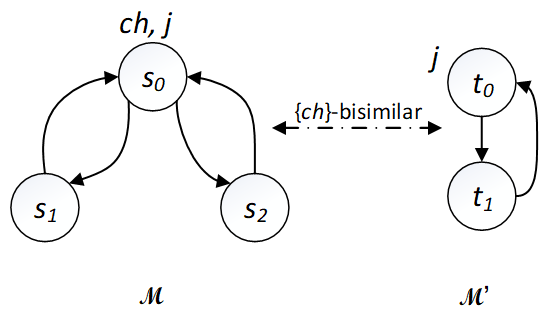
\includegraphics[width=5cm,height=3cm]{chBisimilar.png}\\
		%\vspace{2mm}
		\parbox[c]{6cm}{\footnotesize{Fig.1.~}  Two $\{ch\}$-bisimilar Kripke structures.}%\vspace*{.2mm}
	\end{center}
	
	
\end{example}

Moreover, we can see that the relation $\lrto_V$ has some interesting properties in addition to the equivalence relation. Formally:

\begin{proposition} \label{pro:EqUnion}
	Let $V, V_1 \subseteq \Ha$ and $\Hm_1$, $\Hm_2$ and $\Hm_3$ be three Kripke structures, then we have:
	\begin{enumerate} [(i)]
		\item $\lrto_V$ is an equivalence relation between Kripke structures;
		\item if $\Hm_1 \lrto_V \Hm_2$ and $\Hm_2 \lrto_{V_1} \Hm_3$, then $\Hm_1 \lrto_{V \cup V_1} \Hm_3$.
	\end{enumerate}
	
\end{proposition}

Intuitively, property (i) in Proposition~\ref{pro:EqUnion} means that $\lrto_V$ is reflexive, symmetric, and transitive.
(ii) indicates that if a Kripke structure is $V$ and $V_1$-bisimilar to the other two Kripke structures respectively, then those two Kripke structures are $V \cup V_1$-bisimilar.
As we will show in the following context, it is important to demonstrate the \emph{modularity}, one of the important properties of forgetting in $\mu$-calculus.

%Moreover, as was stated in~\cite{d1996uniform} that any ${\cal L}$-sentence $\varphi$ (that is, a $\mu$-sentence
%that uses only symbols from the language ${\cal L}$) is invariant for ${\cal L}$-bisimulation,  i.e., if there is an ${\cal L}$-bisimulation between $\Hm$ and $\Hm'$, then $\varphi$ holds in $\Hm$ iff it holds in $\Hm'$.
%In this case, it should then be apparent that if $\IR(\varphi, V)$ and
%$\Hm \lrto_V \Hm'$, then $\varphi$ holds in $\Hm$ iff it holds in $\Hm'$.
%In this paper, we call this property \emph{$V$-invariant}.


We now define forgetting in $\mu$-calculus.

\begin{definition}[Forgetting]\label{def:V:forgetting}
	Let $V\subseteq\cal A$ and $\phi$ be a $\mu$-sentence.
	A $\mu$-sentence $\psi$ with $\Var(\psi)\cap V=\emptyset$
	is a {\em result of forgetting $V$ from} $\phi$ if
	\begin{equation*}
		\Mod(\psi)=\{\Hm  \mid \exists \Hm' \in\Mod(\phi)\ \&\ \Hm' \lrto_V \Hm\}.
	\end{equation*}
\end{definition}

%For convenience, we denote the result of forgetting $V$ from $\phi$ as $\Muforget(\phi, V)$.
We denote the result of forgetting $V$ from $\phi$ as $\Muforget(\phi, V)$.
It is not difficult to see that Definition~\ref{def:V:forgetting} implies that if both $\psi$ and $\psi'$ are results of forgetting $V$ from $\phi$, then
$\Mod(\psi)=\Mod(\psi')$, i.e., $\psi$ and $\psi'$ have the same models. In this sense, the result of  forgetting $V$ from $\phi$ is unique up to semantic equivalence.

It is worthy of note that D'Agostino at al. studied the notion of \emph{uniform interpolation} in $\mu$-calculus, and inicated that $\mu$-calculus has the uniform interpolation property~\cite{d1996uniform,d2006modal}. Informally, this means that for every $\mu$-sentence $\varphi$ and every finite set $V\subseteq \Var(\varphi)$, there exists a $\mu$-sentenc $\widetilde{\exists}V \varphi$ which does not contain atoms from $V$ but is logically closest to $\varphi$ in some sense.

We should mention that our forgetting definition $\Muforget(\phi, V)$ is equivalent to the semantic definition of the formula of uniform interpolation in~\cite{d2006modal}.

\subsection{Semantic Properties of Forgetting in $\mu$-calculus}
In this part, we show the semantic properties of forgetting in $\mu$-calculus. In particular, we show that our forgetting is closed in $\mu$-calculus. Moreover, we demonstrate that the notion of forgetting satisfies the general postulates, i.e., the \emph{representation theorem}, and the algebraic properties, including modularity, commutativity, and homogeneity.

%\subsubsection{Characterizing Properties}
It has been proved that the $\mu$-calculus has uniform interpolation~\cite{d2000logical,d1996uniform}. Now, we show that the forgetting in $\mu$-calculus is \emph{closed}~\footnote{Intuitively, given a logic language ${\cal L}$, we say some operator ${\cal O}$ in ${\cal L}$ is closed whenever the result of using the ${\cal O}$ on the elements of ${\cal L}$ is also in ${\cal L}$.}. Formally:

\begin{theorem} \label{thm:exist}
Let $q \in \cal A$ and $\phi$ be a $\mu$-sentence. There is a $\mu$-sentence $\psi$ such that $\IR(\psi, \{q\})$ and $\psi \equiv \Muforget(\phi, \{q\})$.
\end{theorem}

Theorem~\ref{thm:exist} means that the result of forgetting some set of atoms from a $\mu$-sentence is also a $\mu$-sentence; that is, the forgetting in $\mu$-calculus is \emph{closed}.



A general description is important for understanding the concept of forgetting.
To achieve this, four postulates (also called \emph{forgetting postulates}), which indeed precisely characterize the underlying knowledge forgetting semantics  \SFive\ modal logic, is proposed~\cite{Yan:AIJ:2009}.
In the following, we first list these postulates and then show that it also provides an “if and only if” characterization on our notion of forgetting in $\mu$-calculus.

\textbf{Forgetting postulates}~\cite{Yan:AIJ:2009} are:
\begin{itemize}
  \item[] (\W) Weakening: $\varphi \models \varphi'$;
  \item[] (\PP) Positive Persistence:
  for any formula $\eta$, if $\IR(\eta, V)$ and $\varphi \models \eta$ then $\varphi' \models \eta$;
  \item[] (\NgP) Negative Persistence :  for any formula $\eta$,  if $\IR(\eta, V)$ and $\varphi \not \models \eta$ then $\varphi' \not \models \eta$;
  \item[] (\textbf{IR}) Irrelevance: $\IR(\varphi', V)$
\end{itemize}
where $V\subseteq\cal A$,
$\varphi$ is a $\mu$-sentence and $\varphi'$ is the result of
forgetting $V$ from $\varphi$.
%lets explain them here
%
We prefer to list those properties all to outline the basic intuition of forgetting, although they are not all independent,  e.g., (\NgP) is a consequence of (\W) and (\PP).
Intuitively, the postulate (\W) states that forgetting weakens the original formula, i.e., $\varphi'$ is a logical consequence of $\varphi$; the postulates  (\PP) and (\NgP)
state that the forgetting results have no effect on formulas that are independent of the atoms to be forgotten; and the postulate (\textbf{\IR}) states that the
forgetting result is irrelevant to forgotten atoms.

% It is noteworthy that they are not all orthogonal  e.g., (\NgP) is a consequence of (\W) and (\PP). Nonetheless, we prefer to list them all, in order to outline the basic intuition behind them.



The following theorem states that the forgetting postulates above indeed precisely characterize the underling forgetting semantics of $\mu$-calculus.
\begin{theorem}[Representation Theorem]\label{thm:Rep}
Let $\varphi$, $\varphi'$ and $\phi$ be $\mu$-sentences and $V \subseteq \Ha$.
Then the following statements are equivalent:
\begin{enumerate}[(i)]
  \item $\varphi' \equiv \Muforget(\varphi, V)$,
  \item $\varphi'\equiv \{\phi \mid\varphi \models \phi \text{ and } \IR(\phi, V)\}$,
  \item Postulates (\W), (\PP), (\NgP) and (\textbf{IR}) hold if $\varphi,   \varphi'$ and $V$ are as in (i) and (ii).
\end{enumerate}
\end{theorem}
\begin{proof}
$(i) \LRto (ii)$. To prove this, we will show that:
\begin{align*}
 & \Mod(\Muforget(\varphi, V)) = \Mod(\{\phi | \varphi \models \phi, \IR(\phi, V)\}).
\end{align*}
$(\Rto)$ For each model $\Hm'$ of $\Muforget(\varphi, V)$\\
$\Rto$ there exists a Kripke structure $\Hm$ such that $\Hm \models \varphi$ and $\Hm \lrto_V \Hm'$ \hfill (Def. ~\ref{def:V:forgetting}) \\
$\Rto$ $\Hm' \models \phi$ for all $\phi$ with $\varphi \models \phi$ and $\IR(\phi, V)$ \\
$\Rto$ $\Hm' \models \{\phi | \varphi \models \phi, \IR(\phi, V)\}$

$(\Lto)$ It is evident that $\{\phi \mid \varphi \models \phi, \IR(\phi, V)\} \models \Muforget(\varphi, V)$ since $\IR(\Muforget(\varphi, V),V)$ and $\varphi \models \Muforget(\varphi, V)$ by Theorem~\ref{thm:exist}.

$(ii) \Rto (iii)$. For convenience, let $A = \{\phi | \varphi \models \phi, \IR(\phi, V)\}$. Firstly, is easy to see that $\IR(A,V)$ since for any $\phi' \in A$ there is $\IR(\phi',V)$.
Therefore, we have $\IR(\varphi', V)$. Second, $\varphi \models \phi'$ for any $\phi'\in A$, hence $\varphi \models \varphi'$.
%The (\NgP) and (\PP) are obvious from $A$.
Third, $\forall \phi$ with $\IR(\phi, V)$, if $\varphi \models \phi$ then $\phi \in A$ by the definition of $A$. And hence, $\varphi' \models \phi$.
Last but not least, $\forall \phi$ with $\IR(\phi, V)$, if $\varphi \not \models \phi$ then $\phi \not \in A$ by the definition of $A$. And hence, $\varphi' \not \models \phi$ by Definition~\ref{def:V:forgetting} and $V$-invarianty.

$(iii) \Rto (ii)$. (1) $\varphi' \models \{\phi | \varphi \models \phi, \IR(\phi, V)\}$  \hfill ((\PP))\\
  (2) $\{\phi | \varphi \models \phi, \IR(\phi, V)\} \models \varphi'$ \hfill ((\W) and (\textbf{IR}))\\
   $\Rto$ $\varphi'\equiv \{\phi \mid\varphi \models \phi \text{ and } \IR(\phi, V)\}$ \hfill ((1) and (2)).
\end{proof}

Theorem~\ref{thm:Rep}  means that for a given $\mu$-sentence $\varphi$ and a set of atoms $V$, a $\mu$-sentence $\varphi'$ represents a result of forgetting $V$ from $\varphi$ if $\varphi'$ satisfies the forgetting postulates, and vice versa. That is, the representation theorem gives an ``if and only if" characterization on forgetting in $\mu$-calculus, which is in accordance with that in \SFive\ and that in \CTL.

As we mentioned in Related work, the notion of forgetting has been defined and used
in a variety of contexts under PL. It is important to know
the relationship between forgetting in PL and
forgetting in $\mu$-calculus.

To show this, let us recall the following notations for a given atom $p$, a set $V \subseteq \Ha$ of atoms and a PL formula $\varphi$:
$\Forget(\varphi, \{p\})\equiv \varphi[p/\bot] \vee \varphi[p/\top]$ is a result of forgetting $p$ from $\varphi$, and $\Forget(\varphi, V\cup \{p\})$ is recursively defined as $\Forget(\Forget(\varphi, \{p\}),V)$, with $\Forget(\varphi, \emptyset) = \varphi$.
Using this insight, the following result shows that the notion of forgetting (for PL ~\cite{lin1994forget}) is a special case of forgetting in $\mu$-calculus.

\begin{theorem}\label{thm:PL:CTL}
Let $\varphi$ be a PL formula and $V\subseteq \Ha$, then
\[
\Muforget(\varphi, V) \equiv \Forget(\varphi, V).
\]
\end{theorem}

Theorem~\ref{thm:PL:CTL} reveals that the forgetting in $\mu$-calculus is an extension of the forgetting in PL.
This gives us a sense that some of the properties of forgetting in PL also exist in forgetting of $\mu$-calculus.
The following properties hold in PL, modal logic \SFive~\cite{Yan:AIJ:2009} and \CTL~\cite{renyansfirstpaper}. Below we show that they are also satisfied in our notion of forgetting in $\mu$-calculus.

\begin{proposition}
\label{pro:ctl:forget:1}
 Let $\varphi$, $\varphi_i$, $\psi_i$ ($i=1,2$) be $\mu$-sentences and $V\subseteq \Ha$. We have
 \begin{enumerate}[(i)]
   \item $\Muforget(\varphi, V)$ is satisfiable iff $\varphi$ is;
   \item If $\varphi_1 \equiv \varphi_2$, then $\Muforget(\varphi_1, V) \equiv \Muforget(\varphi_2, V)$;
   \item If $\varphi_1 \models \varphi_2$, then $\Muforget(\varphi_1, V) \models \Muforget(\varphi_2, V)$;
   \item $\Muforget(\psi_1 \vee \psi_2, V) \equiv \Muforget(\psi_1, V) \vee \Muforget(\psi_2, V)$;
   \item $\Muforget(\psi_1 \wedge \psi_2, V) \models \Muforget(\psi_1, V) \wedge \Muforget(\psi_2, V)$;
  % \item If $\IR(\psi_1, V)$, then $\Muforget(\varphi \wedge \psi_1, V) \equiv \Muforget(\varphi, V) \wedge \psi_1$.
 \end{enumerate}
\end{proposition}

Intuitively, in Proposition~\ref{pro:ctl:forget:1}, (i) means that forgetting some set of atoms from a sentence does not affect the satisfiability of this sentence. In (ii), we can see that if two sentences are equivalent, then the results of forgetting the same set of atoms from both of them are also equivalent. The intuitive meaning of (iii) is obvious. (iv) indicates that the result of forgetting $V$ from a disjunctive formula $\varphi_1 \vee \varphi_2$ is equivalent to the disjunction of the results of forgetting $V$ from $\varphi_1$ and $\varphi_2$. (v) points out that (iv) is not true for the case of conjunctive formula.

%\subsubsection{Other Semantic Properties}

Postulate (\textbf{IR}) is also of crucial importance for computing the SNC and WSC, in addition to the representation theorem. Consider the $\mu$-sentence $\psi = \varphi \wedge (q \lrto \alpha)$. If $\varphi \wedge \alpha$ is $\{q\}$-irrelevant, then the result of forgetting $q$ from $\psi$ is $\varphi$. Formally, this can be described as in the following lemma, and as we will  see later in Section 4, it is the basis of reducing the SNC (WSC) of any $\mu$-sentence to that of a proposition.

\begin{lemma}
\label{lem:KF:eq}
Let $\varphi$ and $\alpha$ be two $\mu$-sentences and $q\in 	\overline{\Var(\varphi) \cup \Var(\alpha)}$. Then,
 	$\Muforget(\varphi \wedge (q\lrto\alpha), q)\equiv \varphi$.
\end{lemma}

 We will list other interesting properties of the forgetting operator in the following.
 Most importantly, the following property guarantees that we can modularly apply forgetting one by one to the atoms to be forgotten, instead of forgetting the set of atoms as a whole, which is stated in the definition of forgetting.


 \begin{proposition}[Modularity]\label{disTF}  Given a $\mu$-sentence $\varphi$, a set of atoms $V$ and an atom $p$ such that $p \notin V$, then,
 \[
 \Muforget(\varphi, \{p\} \cup V) \equiv \Muforget(\Muforget(\varphi, p), V).
 \]
 \end{proposition}

The next property follows from the above proposition.

\begin{corollary}[Commutativity]\label{disTFV}
Let $\varphi$ be a $\mu$-sentence and $V_i\subseteq{\cal A}~(i=1,2)$. Then,
\[
\Muforget(\varphi, V_1 \cup V_2) \equiv \Muforget(\Muforget(\varphi, V_1), V_2).
\]
\end{corollary}

Another important property of $\Muforget$ is about the formulas with that all the sub-formulas appear in the scope of the same temporal operators $\ALL\NEXT$ or $\EXIST \NEXT$. Formally:


\begin{proposition}[Homogeneity]\label{pro:mu:forget:2}
 Let $V\subseteq\cal A$ and $\phi$ be a $\mu$-sentence; then, we have % and $Q\in \{\EXIST, \ALL\}$.
   \begin{enumerate}[(i)]
     \item $\Muforget(\ALL\NEXT\phi,V)\equiv \ALL\NEXT \Muforget(\phi,V)$.
     \item $\Muforget(\EXIST\NEXT\phi,V)\equiv\EXIST\NEXT \Muforget(\phi,V)$.
   \end{enumerate}
\end{proposition}

The homogeneity of $\ALL\NEXT$ (or $\EXIST\NEXT$) on forgetting indicates that we can move the operator $\Muforget$ afterward to the $\ALL\NEXT$ (or $\EXIST\NEXT$) to forget a set $V$ from a formula in the form $\ALL\NEXT \varphi$ (or $\EXIST\NEXT \varphi$).
%It offers convenience for computing the forgetting.
Especially, when the formula $\phi$ in Proposition~\ref{pro:mu:forget:2} is a PL formula, then forgetting of formulas with the form
$Q\NEXT \phi$ $(Q\in \{\EXIST, \ALL\})$ can be achieved through the corresponding forgetting in PL.

\subsection{Complexity Results}
Computational complexity theory focuses on classifying computational problems according to their resource usage, and relating these classes to each other.
A problem is regarded as inherently difficult if its solution requires significant resources.
Hence, classifying the forgetting operator from its complexity is important to explore an efficient algorithm to compute it.
In this section, we explore the complexity of the forgetting operator from both its model checking and reasoning problems.

Recall that the uniform interpolant $\widetilde{\exists}p \varphi$ ($p\in \Ha$) of a disjunctive $\mu$-formula $\varphi$ is equivalent to the $\mu$-formula $\varphi[p/\top,\neg p/\top]$, where $\varphi[p/\top,\neg p/\top]$ is defined from $\varphi$ by simultaneously substituting the literals $p$ and $\neg p$ with $\top$~\cite{d2006modal}.
Moreover, as we have talked above, our forgetting definition $\Muforget(\varphi, V)$ is equivalent to the semantic definition of uniform interpolant $\widetilde{\exists}V \varphi$\cite{d2006modal}. 
Therefore, the following result is trivial.
\begin{proposition}
 Let $\varphi$ be a $\mu$-sentence and $p\in \Ha$. If $\varphi$ is a disjunctive $\mu$-formula, then $\Muforget(\varphi, \{p\})$ can be computed in linear time.
 \end{proposition}
 %\begin{proof}
% By Theorem~\ref{thm:disUniF} and Theorem~\ref{thm:exist}, we have $\Muforget(\varphi, \{p\}) \equiv \varphi[p/\top, \neg p/\top]$, where $\varphi[p/\top$, $\neg p/\bot]$ is obtained from $\varphi$ by simultaneously
%substituting the literals $p$ and $\neg p$ with $\top$.
% \end{proof}



In this sense, we can transform a formula into its disjunctive form offline and then compute the result of forgetting some atoms from it, which will be efficient in some situations.
 %Let's recall the three disjunctive formulas, which obtained from  $\mu$-sentences, in Example~\ref{exmp:disF}.
In the following example, we show how to compute forgetting ``$ch$" from those disjunctive $\mu$-formulas.

 \begin{example}
 Let us consider the following formulas:
$\varphi_1=  j \wedge ch \wedge Cover(\neg j \wedge \neg ch, \top),$ $ \varphi_2= \mu X. (j \wedge ch) \wedge Cover(X, \top)$ and $\varphi_3=  \nu X. (j \wedge ch) \wedge Cover(Cover(X,$ $\top), \top)$. Let $V=\{ch\}$, we can easily compute the results of forgetting $V$ from these formulas.

(1) $\Muforget(\varphi_1, V) \equiv j \wedge Cover(\neg j, \top) \equiv j \wedge \EXIST \NEXT(\neg j)$;

(2) $\Muforget(\varphi_2, V) \equiv \mu X. j  \wedge Cover(X, \top) \equiv \mu X. j \wedge \EXIST \NEXT X$;

(3) $\Muforget(\varphi_2, V) \equiv \nu X. j \wedge Cover(Cover(X, \top), \top) \equiv \nu X. j \wedge \EXIST \NEXT(\EXIST \NEXT X)$.
 \end{example}


Nevertheless, we will show that the model checking problem of forgetting is intractable even if the given formula is a disjunctive formula.

\begin{proposition}[Model Checking]\label{pro:MC}
Given a finite Kripke structure  $\Hm$, a $\mu$-sentence $\varphi$ and $V\subseteq \Ha$. We have:
\begin{itemize}
  \item[(i)] Deciding $\Hm \models^? \Muforget(\varphi, V)$ is $\textsc{Exptime}$;
  \item[(ii)] If $\varphi$ is a disjunctive $\mu$-formula, then deciding $\Hm \models^? \Muforget(\varphi, V)$ is in \textsc{NP}$\cap$co-\textsc{NP}.
\end{itemize}
\end{proposition}

More importantly, from the perspective of knowledge base evolution,
the following reasoning problems about forgetting, which are explored in PL~\cite{wang2015forgetting}, are also of interest.
%we are also interested in the following reasoning problems about forgetting, which are explored in CPL~\cite{wang2015forgetting}:

\begin{enumerate}[(i)]
    \item $[$Var-weak$]$ if the restriction of $\varphi$ on the signature of $\psi$ is at most as strong as $\psi$, i.e., $\psi\models \Muforget(\varphi, V)$,
    \item $[$Var-strong$]$ if the restriction of $\varphi$ on the signature of $\psi$ is at least as strong as $\psi$, i.e., $\Muforget(\varphi, V)\models \psi$,
    \item $[$Var-entailment$]$ if the restriction of one knowledge base on its original signature is at most as strong as that of the other, i.e., $\Muforget(\varphi, V) \models \Muforget(\psi, V)$
\end{enumerate}
where $\varphi$, $\psi$ are $\mu$-sentences, and $V$ is a set of atoms. In addition, in (i) and (ii), there is $\Var(\varphi) - V = \Var(\psi)$, and in (iii), there is $V \subseteq \Var(\varphi) \cap \Var(\psi)$. Then, we have the following results.


\begin{theorem}[Entailment]
	\label{thm:Ent}
Let $\varphi$ and $\psi$ be two $\mu$-sentences and $V$ be a set of atoms. Then, the following problems are $\textsc{Exptime}$-complete.
\begin{enumerate}[(i)]
  \item deciding  $\Muforget(\varphi, V ) \models^? \psi$,
  \item deciding  $\psi \models^? \Muforget(\varphi, V)$,
  \item deciding $\Muforget(\varphi, V) \models^? \Muforget(\psi, V)$.
\end{enumerate}
\end{theorem}
%\begin{proof}
%We prove the (i), there other two results can be proved similarly.
%
%Let $A_{\varphi}$ and $A_{\psi}$ be the $\mu$-automaton of $\varphi$ and $\psi$ respectively, we can construct the $\mu$-automaton $B$ of $\Muforget(\varphi, V )$ from $A_{\varphi}$ by the proof of Proposition~\ref{pro:MC}. By Proposition 7.3.2 in~\cite{comon1997tree}
%, we can obtain the complement $C$ of $A_\psi$ in linear time, and then the intersection $A_{C \cap B}$ between $C$ and $B$  in linear time. In this case, the $\Muforget(\varphi, V ) \models^? \psi$ is reduced to decide whether the language accepted by $A_{C \cap B}$ is empty, which is $\textsc{Exptime}$-complete~\cite{comon1997tree}.
%\end{proof}

Similar to the reasoning problems discussed above, the following equivalent problems are also important, in which ``var-independence" and ``var-equivalence" under PL are proposed in~\cite{lang2003propositional}:
\begin{enumerate}[(i)]
    \item $[$Var-independence$]$ if a formula $\varphi$ is independent of a set $V$ of atoms, i.e., $\Muforget(\varphi,V) \equiv \varphi$,
    \item $[$Var-match$]$ if the restriction of $\varphi$ on the signature of $\psi$ perfectly matches $\psi$, i.e., $\Muforget(\varphi, V) \equiv \psi$,
    \item $[$Var-equivalence$]$ if the restriction of the two formulas on a common signature are equivalent, i.e., $\Muforget(\varphi, V) \equiv \Muforget(\psi, V)$.
\end{enumerate}

The following results are implications of Theorem~\ref{thm:Ent}.

\begin{corollary}\label{cor:equiv}
Let $\varphi$ and $\psi$ be two $\mu$-sentences and $V$ be a set of atoms. Then, the following problems are $\textsc{Exptime}$-complete.
\begin{enumerate}[(i)]
  \item deciding $\psi \equiv^?\Muforget(\varphi, V)$,
  \item deciding $\Muforget(\varphi, V) \equiv^? \varphi$,
  \item deciding $\Muforget(\varphi, V) \equiv^? \Muforget(\psi, V)$.
\end{enumerate}
\end{corollary}


\section{Applications of Forgetting}\label{applications}
As mentioned above, forgetting in PL has been used in a variety of contexts, we show how forgetting in $\mu$-calculus can be used in computing WSC (SNC) and knowledge update in this section.

\subsection{Necessary and Sufficient Conditions}\label{ns_conditions}
In this section, we present two key notions of our work:  the SNC and the WSC  of a given $\mu$-calculus specification, which correspond to the \emph{most general consequence} and the \emph{most specific abduction} of a specification, respectively.  As mentioned in the introduction, these notions are in accordance with the SP and the WP (introduced by E. Dijkstra in \cite{DBLP:journals/cacm/Dijkstra75}), which have been central to a wide variety of tasks and studies, e.g. generating counterexamples and refining system in verification. Our contribution, in particular, will be to compute the SNC and WSC by forgetting under a given $\mu$-sentence and a set $V$ of atoms.  Let us give the formal definition.

\begin{definition}[sufficient and necessary condition]\label{def:NC:SC}
Let $\phi$, $\psi$ be two $\mu$-sentences, $V \subseteq \Var(\phi)$, $q\in\Var(\phi)- V$
and $\Var(\psi)\subseteq V$.
\begin{itemize}
  \item $\psi$  is a {\em necessary condition} (NC) of $q$ on $V$ under $\phi$
    if $\phi \models q \rto \psi$.
  \item $\psi$  is a {\em sufficient condition} (SC) of $q$ on $V$ under $\phi$
    if $\phi \models \psi\rto q$.
  \item $\psi$  is a {\em strongest necessary condition} (SNC in short)
  of $q$ on $V$ under $\phi$
    if it is an NC of $q$ on $V$ under $\phi$, and $\phi\models\psi\rto\psi'$
    for any NC $\psi'$ of $q$ on $V$ under $\phi$.

    \item $\psi$  is a {\em weakest sufficient condition} (WSC in short)
  of $q$ on $V$ under $\phi$
    if it is an SC of $q$ on $V$ under $\phi$, and $\phi\models\psi'\rto\psi$
    for any SC $\psi'$ of $q$ on $V$ under $\phi$.
\end{itemize}
\end{definition}

Intuitively, the SNC (WSC) is the strongest (weakest) among the NCs (SCs) of $q$ on $V$ under $\phi$, i.e., for each $\psi'$ with $\phi \models q \rto \psi'$ ($\phi \models \psi' \rto q$), $\phi \models \hbox{SNC} \rto \psi'$ ($\phi \models \psi' \rto \hbox{WSC}$).
Note that if both $\psi$ and $\psi'$ are SNCs (WSCs) of $q$ on $V$ under $\phi$, then
$\psi\equiv \psi'$. %, i.e., they are the  logical consequences of each other.
In this sense, the SNC (WSC) of $q$ on $V$ under $\phi$ is unique (up to semantic equivalence). Furthermore, the following result shows that the SNC and WSC are dual notions.

\begin{proposition}[Dual]\label{dual}
 Let $V,q,\varphi$ and $\psi$ be defined as in Definition~\ref{def:NC:SC}.
 Then, $\psi$ is an SNC (a WSC) of $q$ on $V$ under $\varphi$ iff $\neg \psi$ is a WSC (an SNC)
    of $\neg q$ on $V$ under $\varphi$.
\end{proposition}


Replacing $q$ with any $\mu$-sentence $\alpha$ and redefining $V$  as a subset of $\Var(\alpha) \cup \Var(\phi)$ in Definition~\ref{def:NC:SC}, we can generalize this definition to arbitrary formulas.

It turns out that we can lift previous concepts of the SNC and WSC for an  atomic variable to any formula or, on the contrary, reduce the SNC and WSC of any formula to that of an atomic variable, as shown in the following results.


\begin{proposition}\label{formulaNS_to_p}
     Let $\Gamma$ and $\alpha$ be two $\mu$-sentences, $V \subseteq \Var(\alpha) \cup \Var(\Gamma)$  and $q$ be a new proposition not in $\Gamma$ and $\alpha$.
 Then, a formula $\varphi$ with $\Var(\varphi) \subseteq V$ is the SNC (WSC) of $\alpha$ on $V$ under  $\Gamma$ iff it is the SNC (WSC) of $q$ on $V$ under $\Gamma' = \Gamma \cup \{q \lrto \alpha\}$.
 \end{proposition}


The following result shows that the forgetting and notion of the SNC (WSC) are closely related.%, which are central to our contribution.

\begin{theorem}\label{thm:SNC:WSC:forget}
 Let $\varphi$ be a $\mu$-sentence, $V\subseteq\Var(\varphi)$ and $q\in\Var(\varphi)- V$.
 \begin{enumerate}[(i)]
   \item $\Muforget(\varphi \land q$, $(\Var(\varphi) \cup \{q\}) - V)$
   is a SNC of $q$ on $V$ under $\varphi$.
   \item  $\neg\Muforget (\varphi \land \neg q$, $(\Var(\varphi) \cup \{q\}) - V)$
   is a WSC of $q$ on $V$ under $\varphi$.
 \end{enumerate}
 \end{theorem}
 \begin{proof}
  We will prove the SNC part, while it is not difficult to prove the WSC part according to Proposition \ref{dual}. And let ${\cal F}=\Muforget(\varphi \wedge q, (\Var(\varphi) \cup \{q\})- V)$.

    The ``NC" part: It's easy to see that $\varphi \wedge q \models {\cal F}$ by {\bfseries (W)}. Hence, $\varphi\models q \rto {\cal F}$, this means
  ${\cal F}$ is a NC of $q$ on $V$ under $\varphi$.

  The ``SNC" part: We shall show that for all $\psi'$ with $\psi'$ is the NC of $q$ on $V$ under $\varphi$, i.e. $\varphi \models q \rto \psi'$ and $\Var(\psi') \subseteq V$, there is $\varphi \models {\cal F} \rto \psi'$. Suppose that there exists a NC $\psi$ of $q$ on $V$ under $\varphi$ with $\psi$ is not logic equivalence with ${\cal F}$ under $\varphi$, such that $\varphi \models \psi \rto {\cal F}$.\\
  $\Rto$ $\varphi \wedge q \models \psi$ iff ${\cal F} \models \psi$ \hfill ((\PP) and $\IR(\psi, (\Var(\varphi)\cup \{q\})) -V$)\\
  $\Rto$ $\varphi \wedge {\cal F} \models \psi$  \hfill ($\varphi \wedge q \models \psi$ (by suppose))\\
  $\Rto$ $\varphi \wedge \psi \models {\cal F}$  \hfill (by suppose)\\
  $\Rto$ $\varphi \models \psi \lrto {\cal F}$  \hfill (Contradict with the suppose)

  Therefore, ${\cal F}$ is the SNC of $q$ on $V$ under $\varphi$.
 \end{proof}
%
%Following Theorem~\ref{thm:SNC:WSC:forget}, assume that $\psi = \Muforget(\varphi \wedge q, (\Var(\varphi) \cup \{q\})- V)$.  Then, $\varphi \wedge q \models \psi$  by (\W). Moreover,  $\varphi \wedge q \models \psi$,  and then, $\psi$ is an NC of $q$ on $V$ under $\varphi$.
%
%In addition, for any $\mu$-sentence $\psi'$ with $\IR(\psi', (\Var(\varphi) \cup \{q\})- V)$ and $\varphi \wedge q \models \psi'$,
%we have $\psi \models \psi'$ by (\PP). Therefore, $\psi$ is the SNC of $q$ on $V$ under $\varphi$, which shows the intuition of how the SNC can be obtained from the forgetting.

Recall that any initial $\MPK$-structure  can be expressed as a \CTL\ formula~\cite{renyansfirstpaper}.
In this sense, when the given system $\Hm$ is an initial $\MPK$-structure, it is easy to compute the WSC of $\varphi$ on some set of atoms under $\Hm$ in the model checking problem $\Hm \models \varphi$ by using forgetting.

Another important point is that although we can use forgetting to compute the SNC and WSC, it has been found that sometimes, it is much easier
to compute the SNC than the WSC, and
sometimes, it is the other way around~\cite{DBLP:Lin:AIJ:2001}. For instance, the author found that for many
formulas, the SNCs are easier to compute than WSCs~\cite{DBLP:Lin:AIJ:2001}. Therefore, when one condition is much easier to compute, the following proposition will
be very helpful in computing the other condition.

\begin{proposition}\label{pro:eachOne}
Let $\Gamma$ be a $\mu$-sentence, $q$ be a proposition, and $V$ be a set of propositions.
\begin{enumerate}[(i)]
 \item If $\varphi$ is an NC of $q$ on $V$ under $\Gamma$, and $\psi$ is the WSC of $q$ on $V$ under $\Gamma \cup \{\varphi\}$, then $\varphi \wedge \psi$ is the WSC of $q$ on $V$ under $\Gamma$.
 \item  If $\psi$ is an SC of $q$ on $V$ under $\Gamma$ and $\varphi$ is the SNC of $q$ on $V$ under $\Gamma \cup \{\neg \psi\}$, then $\varphi \vee \psi$ is the SNC of $q$ on $V$ under $\Gamma$.
 \end{enumerate}
\end{proposition}



Even so,  deciding whether a $\mu$-sentence $\psi$ is an SNC (a WSC) of the given $q$ on a set $V$ of atoms under $\mu$-sentence $\varphi$ is intractable since the problem of deciding whether $\varphi \models q \rto \psi$ is $\textsc{Exptime}$-complete~\cite{bradfield2018mu}.
Thus, deciding whether $\psi$ is an NC of $q$ on $V$ under $\varphi$ is $\textsc{Exptime}$-complete.
Formally, we have the following result.
\begin{theorem}\label{thm:exp:snc}
Let $\psi$ and $\varphi$ be two $\mu$-sentences, $V\subseteq \Var(\varphi)$ be a set of atoms, $q \in \Var(\varphi) - V$ and $\Var(\psi) \subseteq V$. Then, the following problems are $\textsc{Exptime}$-complete.
\begin{enumerate}[(i)]
    \item Deciding whether $\psi$ is an SNC of $q$ on $V$ under $\varphi$,
    \item Deciding whether $\psi$ is a WSC of $q$ on $V$ under $\varphi$.
\end{enumerate}
\end{theorem}



\subsection{Representing a Knowledge Update Via Forgetting}\label{knowledge_updat}
As talked in Introduction, knowledge update, originates from belief revision and update, has been defined by knowledge forgetting in S5 modal logic~\cite{Zhang2009Knowledge}.
This section presents the final key notion of our work: the knowledge update.
Similarly, we propose a method of defining knowledge update by forgetting in $\mu$-calculus that will
satisfy all the following Katsuno and Mendelzon's postulates (U1)-(U8) proposed in~\cite{katsuno91mendelzon}:
\begin{enumerate}[]
    \item (U1)  $\Gamma \diamond \phi \models \phi$.
    \item (U2) If  $\Gamma \models \phi$,  then  $\Gamma \diamond \phi \equiv \Gamma$.
    \item (U3) If both $\Gamma$ and $\phi$ are satisfiable, then $\Gamma \diamond \phi$ is also satisfiable.
    \item (U4) If $\Gamma_1\equiv \Gamma_2$ and $\phi_1 \equiv \phi_2$, then $\Gamma_1 \diamond \phi_1 \equiv \Gamma_2 \diamond \phi_2$.
    \item (U5) $(\Gamma \diamond \phi) \wedge \psi \models \Gamma \diamond(\phi \wedge \psi)$.
    \item (U6) If $\Gamma \diamond \phi \models \psi$ and $\Gamma \diamond \psi \models \phi$, then $\Gamma \diamond \phi \equiv \Gamma \diamond \psi$.
    \item (U7) If $\Gamma$ has a unique model, then $(\Gamma \diamond \phi) \wedge (\Gamma \diamond \psi) \models \Gamma \diamond (\phi \vee \psi)$.
    \item (U8) $(\Gamma_1 \vee \Gamma_2) \diamond \phi \equiv (\Gamma_1 \diamond \phi) \vee  (\Gamma_2 \diamond \phi)$.
\end{enumerate}
where $\varphi \diamond \psi$ expresses the result of updating $\varphi$ with $\psi$ and $\diamond$ is the knowledge update operator.


For this purpose, in this part, we assume that the models of a $\mu$-sentence are initial structures.
%, where an \emph{initial structure} is a Kripke structure $\Hm=(S, sr, R, L)$ with $S$ being a finite set of states, $sr$ being an initial state (i.e., for each state $s'\in S$, the $sr$ can arrive at $s'$), $R$ being a total relation and $L: S \rto 2^{\Ha}$ being a label function, where $\Ha$ is restricted to a finite set.
In addition, we also limit the definition of forgetting on initial structures,
i.e., the models mentioned in Definition~\ref{def:V:forgetting} are initial structures. In this case, we have:

%限制模型的情形
\begin{theorem}\label{thm:initModel}
Let $V \subseteq \cal A$ and $\phi$ be a $\mu$-sentence. Then there is a $\mu$-sentence $\psi$ such that:
\[
    \Hm \models \psi \mbox{ iff there exists } \Hm'\in\Mod(\phi) \mbox{ s.t. } \Hm \lrto_V \Hm' % \mbox{ and } \Hm' \models \phi.
\]
where both $\Hm$ and $\Hm'$ are initial structures.
\end{theorem}

%Intuitively, given a logic language ${\cal L}$, we say some operator ${\cal O}$ in ${\cal L}$ is closed whenever the result of using the ${\cal O}$ on the elements of ${\cal L}$ is also in ${\cal L}$.
Theorem~\ref{thm:initModel} shows that the forgetting in $\mu$-calculus is also closed when restricting the models of the $\mu$-sentence to initial structures. Formally:

\begin{corollary}
The forgetting of $\mu$-calculus is closed under the initial structure semantic, i.e., we consider only the initial structures as the models of the $\mu$-sentence.
\end{corollary}

According to~\cite{renyansfirstpaper}, we can see that any initial structure $\Hm$ on $\Ha$ can be captured by a \CTL\ formula, i.e., the characterizing formula ${\cal F}_{\Ha}(\Hm)$~\cite{renyansfirstpaper}, and hence a $\mu$-sentence~\cite{emerson1997model}.
For the set $\Ha$, $V_{min}$, and $\varphi = \Muforget({\cal F}_{\Ha}(\Hm), V_{min})$, by $\Mod(\varphi)$, we mean the set of models of $\varphi$, where $V_{min} \subseteq \Ha$ is a minimal subset of atoms that makes $\varphi$ consistent.
Besides, $$\bigcup_{V_{min}\subseteq \Ha} \Mod(\varphi)$$ denotes the union of $\Mod(\varphi)$ with $V_{min}\subseteq \Ha$.
Then, we define the knowledge update operator $\diamond_{\mu}$ in $\mu$-calculus as follows.


\begin{definition}\label{def:KU}
  Let $\Gamma$ and $\phi$ be $\mu$-sentences. The knowledge update operator $\diamond_{\mu}$ is defined as follows:
  \[
  \Mod(\Gamma \diamond_{\mu} \phi) = \bigcup_{\Hm \in \Mod(\Gamma)} \bigcup_{V_{min}\subseteq \Ha} \Mod(\Muforget({\cal F}_{\Ha}(\Hm), V_{min}) \wedge \phi),
  \]
  where ${\cal F}_{\Ha}(\Hm)$ is the characterizing  formula of $\Hm$ on $\Ha$ and $V_{min} \subseteq \Ha$ is a minimal subset of atoms that makes $\Muforget({\cal F}_{\Ha}(\Hm), V_{min}) \wedge \phi$ consistent.
\end{definition}

Intuitively, $\Gamma \diamond_{\mu} \phi$ is the result of updating $\Gamma$ with $\phi$ by minimally fixing the models of $\Gamma$ to that of $\phi$.
In other words, the knowledge update defined in Definition~\ref{def:KU} is achieved by minimally changing every model of $\Gamma$ to make it consistent with $\phi$. In this sense, this method can be viewed as a model-based update approach.

Recall the definition of knowledge update in PL:
Let $I$, $J_1$ and $J_2$ be three interpretations; then $J_1$ is closer to $I$ than $J_2$, written $J_1 \leq_{I,pam} J_2$, iff $\Diff(I, J_1) \subseteq \Diff(I, J_2)$, where $\Diff(X, Y) =\{p\in \Ha \mid X(p) \not = Y(p)\}$.
The set of models of knowledge updating $\psi$ on $\Gamma$ is exactly the union of the minimal models of $\psi$ under the partial order $\leq_{I,pam}$, where $I$ is a model of $\Gamma$, i.e., $$\Mod(\Gamma \diamond_{pam} \psi) = \bigcup_{I \in \Mod(\Gamma)} Min(\Mod(\psi), \leq_{I,pam}).$$ Here, $Min(\Mod(\psi), \leq_{I,pam})$ is the set of models of $\psi$ that are minimal with respect to $\leq_{I,pam}$.


Similarly, we define a partial ordering over the set of initial structures that link to the knowledge operator $\diamond_{\mu}$.

\begin{definition}\label{def:closer}
  let $\Hm$, $\Hm_1$ and $\Hm_2$ be three initial structures, then $\Hm_1$ is closer to $\Hm$ than $\Hm_2$, written $\Hm_1 \leq_{\Hm} \Hm_2$, iff for any $V_2 \subseteq \Atom$ such that $\Hm_2 \lrto_{V_2} \Hm$, there exists a $V_1 \subseteq V_2$ such that $\Hm_1 \lrto_{V_1} \Hm$. We denote $\Hm_1 <_{\Hm} \Hm_2$ iff $\Hm_1 \leq_{\Hm} \Hm_2$ and $\Hm_2 \not \leq_{\Hm} \Hm_1$.
\end{definition}

%与2006那个模型更新的minimal作比较

Let $M$ be a set of initial structures and $\Hm$ be an initial structure. We also use $Min(M,$ $\leq_{\Hm})$ to denote the set of all minimal initial structures with respect to $\leq_{\Hm}$.
Then, the following theorem is important for relating $\diamond_{\mu}$ and $\leq_{\Hm}$.
%Then we have the following theorem.


\begin{theorem}\label{thm:minU}
Let $\Gamma$ and $\phi$ be $\mu$-sentences. Then, we have:
\[\Mod(\Gamma \diamond_{\mu} \phi) = \bigcup_{\Hm\in \Mod(\Gamma)} Min(\Mod(\phi), \leq_{\Hm}).
\]
\end{theorem}

Theorem~\ref{thm:minU} indicates that our definition of knowledge update in $\mu$-calculus by forgetting is in accordance with the one defined by the $\leq_{\Hm}$, which is similar to the partial order $\leq_{I, pam}$ in PL.

More importantly, the following theorem shows that our definition of $\diamond_{\mu}$ by forgetting satisfies the Katsuno and Mendelzon update postulates.
\begin{theorem}\label{thm:U1toU8}
The knowledge update operator $\diamond_{\mu}$ satisfies the Katsuno and Mendelzon's update postulates (U1)-(U8).
\end{theorem}


\section{Concluding Remarks}\label{sec:conclude}
\paragraph{Summary}
In this paper, we targeted the strongest necessary and weakest sufficient conditions (SNC and WSC) and knowledge update in $\mu$-calculus using a forgetting-based approach.
In doing so, we introduced and employed the notion of $V$-bisimulation, which is similar to the ${\cal L}$-bisimulation, in which any $\mu$-sentence is invariant for ${\cal L}$-bisimulation.
Furthermore, we studied formal properties about forgetting, including homogeneity, modularity, and commutativity.
In particular, we showed that our notion of forgetting satisfies the well-known forgetting postulates. Thus, it faithfully extends the notion of forgetting in classical propositional logic, modal logic \SFive\  and \CTL.
We also showed that for any $\mu$-sentence, if it is a disjunctive formula, then forgetting a set  of atoms from it can be done in linear time.
From the perspective of computational complexity,
%the complexity theory side,
we investigated whether the model checking problem for forgetting results  from a disjunctive formula is in \textsc{NP}$\cap$co-\textsc{NP}
and whether the entailment problems relating to forgetting are $\textsc{Exptime}$-complete. % from the point of $\mu$-automaton.
Moreover, deciding whether a given $\mu$-sentence is a SNC (WSC) of a specification is $\textsc{Exptime}$-complete.
We finally showed that the knowledge update in terms of forgetting  for $\mu$-calculus
under initial structures satisfies the Katsuno and Mendelzon's postulates (U1)-(U8).

\paragraph{Future work}
In the future, an algorithm to compute forgetting will be explored and implemented. As shown in this work, the forgetting of a disjunctive formula can be done in linear time. In this sense, a method of transforming a formula into its disjunctive form will be useful for the forgetting algorithm.
% As we can see that the model checking problem of forgetting is \textsc{NP} $\cap$ co-\textsc{NP} and the reasoning problems of forgetting are $\textsc{Exptime}$-complete, which means there is no algorithm can compute the result of forgetting a set of atoms from a $\mu$-sentence in polynomial time.
In addition, it is worthwhile to explore sub-classes of $\mu$-calculus for which the forgetting can be computed easily.
Moreover, when a finite transition system $\Hm$ does not satisfy a specification $\varphi$,
it is important to calculate the weakest sufficient condition $\psi$ over a signature $V$ under which $\Hm$ satisfies $\varphi$. %viz. expressing $\Hm$ with its characterizing formula, to explore how the condition $\psi$ can guide the design of a new transition system $\Hm'$ satisfying $\varphi$.
It is also crucial to explore how the weakest sufficient condition $\psi$
can be used to revise or update the transition system $\Hm$ for the specification $\varphi$.


\clearpage
\bibliographystyle{splncs04}
\bibliography{muRef}


\clearpage
\appendix
\section{Supplementary Material: Proof Appendix}

\noindent\textbf{Proposition}~\ref{pro:EqUnion}
Let $V, V_1 \subseteq \Ha$, $\Hm_1$, $\Hm_2$ and $\Hm_3$ be three Kripke structures, then we have:
\begin{enumerate} [(i)]
    \item the $\lrto_V$ is an  equivalence relation between Kripke structures;
    \item if $\Hm_1 \lrto_V \Hm_2$ and $\Hm_2 \lrto_{V_1} \Hm_3$, then $\Hm_1 \lrto_{V \cup V_1} \Hm_3$.
\end{enumerate}
\begin{proof}
(i) We prove it form the reflexivity, symmetry and transitivity.

(1) $\lrto_V$ is reflexive. It is easy to check that $\Hm\lrto_V \Hm$ for any Kripke structure.

(2) $\lrto_V$ is symmetric. We will show that for each $\Hm_1$ and $\Hm_2$, if $\Hm_1 \lrto_V \Hm_2$ then $\Hm_2 \lrto_V \Hm_1$.
Supposing $\Hm_1 \lrto_V \Hm_2$ by the $V$-bisimulation $\Hb$, we construct a relation $\Hb_1$ as follows: $\Hb_1=\{(s,t) | (t, s)\in \Hb\}$. We will show that $\Hb_1$ is a $V$-bisimulation between $\Hm_2$ and $\Hm_1$ from the following several points:
\begin{itemize}
    \item $r_2 \Hb_1 r_1$ since $r_1 \Hb r_2$,
    \item for each $s\in S_1$ and $t\in S_2$, if $t \Hb_1 s$ then we have $s\Hb t$ and hence $p \in L_1(s)$ iff $p \in L_2(t)$ for each $p \in \Ha - V$, and
    \item the third and forth points in the definition of $V$-bisimulation can be checked easily for $\Hb_1$.
\end{itemize}

(3) $\lrto_V$ is transitive. We will show that for each $\Hm_1$, $\Hm_2$ and $\Hm_3$, if $\Hm_1 \lrto_V \Hm_2$ and $\Hm_2 \lrto_V \Hm_3$ then $\Hm_1 \lrto_V \Hm_3$. Supposing $\Hm_1 \lrto_V \Hm_2$ by the $V$-bisimulation $\Hb_1$ and $\Hm_2 \lrto_V \Hm_3$  by the $V$-bisimulation $\Hb_2$, we construct a relation $\Hb$ as follows: $\Hb=\{(s, z) | (s,t) \in \Hb_1\ \mbox{and}\ (t, z)\in \Hb_2\}$.
We can also prove similarly with (2) that $\Hb$ is a $V$-bisimulation between $\Hm_1$ and $\Hm_3$. Therefore, $\Hm_1 \lrto_V \Hm_3$.

(ii) In order to prove $\Hm_1 \lrto_{V\cup V_1} \Hm_3$, we only need to find a binary relation $\Hb$ such that $\Hb$ is a $(V\cup V_1)$-bisimulation between $\Hm_1$ and $\Hm_3$.
Supposing $\Hm_1 \lrto_V \Hm_2$ by the $V$-bisimulation $\Hb_1$ and $\Hm_2 \lrto_{V_1} \Hm_3$  by the $V_1$-bisimulation $\Hb_2$. Let $\Hb = \{(s_1, s_3)| (s_1, s_2) \in \Hb_1\ \mbox{and} \ (s_2, s_3) \in \Hb_2\}$. We can easily check that $\Hb$ is a $(V\cup V_1)$-bisimulation between $\Hm_1$ and $\Hm_3$.


\end{proof}




\noindent\textbf{Theorem}~\ref{thm:exist}
Let $q \in \cal A$ and $\phi$ be a $\mu$-sentence. There is a $\mu$-sentence $\psi$ such that $\IR(\psi, \{q\})$ and $\psi \equiv \Muforget(\phi, \{q\})$.
\begin{proof}
It has been proved that for each $\mu$-sentence $\phi$ and atom $p$, there is a $\mu$-sentence $\phi'$ with $\IR(\phi', \{p\})$ such that (Theorem 3.1 in~\cite{d1996uniform}):
\[
    \Hm \models \phi' \mbox{ iff } \exists \Hm' \in \phi \mbox{ such that } \Hm \lrto_{\{p\}} \Hm'.
\]
This is accordance with the definition of forgetting.
\end{proof}


\noindent\textbf{Theorem}~\ref{thm:PL:CTL}
Let $\varphi$ be a PL formula and $V\subseteq \Ha$, then
\[
\Muforget(\varphi, V) \equiv \Forget(\varphi, V).
\]
\begin{proof}
Let $\Hm = (S, r, R, L)$ and $\Hm' = (S', r', R', L')$ be two Kripke structure.
It is easy to see that a Kripke structure $\Hm$ is a model of a PL formula $\psi$ if $L(r)$ satisfy $\psi$, and also can be denoted as $\Hm \models \psi$.

$(\Rto)$ For each $\Hm \in \Mod(\Muforget(\varphi, V))$ \\
$\Rto$ $\exists \Hm' \in \Mod(\varphi)$ such that $\Hm \lrto_V \Hm'$ by the $V$-bisimulation ${\cal B}$ \hfill(Def. ~\ref{def:V:forgetting})\\
$\Rto$ $r {\cal B} r'$ \\
$\Rto$ $\Hm \models \Forget(\varphi, V)$  \hfill ($\IR(\Forget(\varphi, V),V)$ and $V$-invariant)

$(\Lto)$ For each $\Hm \in \Mod(\Forget(\varphi, V))$ \\
$\Rto$ $\exists \Hm' \in\Mod(\varphi)$ such that for each $p \in \Ha-V$, $p \in L(r)$ iff $p \in L'(r')$ \hfill (by the definition of $\Forget$)\\
%$r {\cal B} r'$\\
$\Rto$ Constructing a Kripke structure $\Hm_1 = (S_1, r_1, R_1, L_1)$ such that:
\begin{itemize}
    \item [*] $S_1 = (S - \{r\}) \cup \{r_1\}$,
    \item [*] $R_1$ is the same as $R$ except that $r$ is replaced by $r_1$, and
    \item [*] $L_1$ is the same as $L$ except $L_1(r_1) = L'(r')$.
\end{itemize}
% $S_1 = (S - \{r\}) \cup \{r_1\}$, $R_1$ is the same as $R$ except that $r$ is replaced by $r_1$, and $L_1$ is the same as $L$ except $L_1(r_1) = L'(r')$. \\
$\Rto$ $\Hm_1 \models \varphi$ and $\Hm_1 \lrto_V \Hm$\\
$\Rto$ $\Hm \models \Muforget(\varphi, V)$ \hfill ($\IR(\Muforget(\varphi, V), V)$ and $V$-invariant)
\end{proof}


\noindent\textbf{Proposition}
\ref{pro:ctl:forget:1}
 Let $\varphi$, $\varphi_i$, $\psi_i$ ($i=1,2$) be formulas in $\mu$-calculus and $V\subseteq \Ha$. We have
 \begin{enumerate}[(i)]
   \item $\Muforget(\varphi, V)$ is satisfiable iff $\varphi$ is;
   \item If $\varphi_1 \equiv \varphi_2$, then $\Muforget(\varphi_1, V) \equiv \Muforget(\varphi_2, V)$;
   \item If $\varphi_1 \models \varphi_2$, then $\Muforget(\varphi_1, V) \models \Muforget(\varphi_2, V)$;
   \item $\Muforget(\psi_1 \vee \psi_2, V) \equiv \Muforget(\psi_1, V) \vee \Muforget(\psi_2, V)$;
   \item $\Muforget(\psi_1 \wedge \psi_2, V) \models \Muforget(\psi_1, V) \wedge \Muforget(\psi_2, V)$;
  % \item If $\IR(\psi_1, V)$, then $\Muforget(\varphi \wedge \psi_1, V) \equiv \Muforget(\varphi, V) \wedge \psi_1$.
 \end{enumerate}
\begin{proof}
 (i) ($\Rto$) Supposing $\Hm$ is a model of $\Muforget(\varphi, V)$, then there is a model $\Hm'$ of $\varphi$ s.t. $\Hm \lrto_V \Hm'$ by the definition of $\Muforget$.

 ($\Lto$) Supposing $\Hm$ is a model of $\varphi$, then there is a Kripke structure $\Hm'$ s.t. $\Hm \lrto_V \Hm'$, and then $\Hm' \models \Muforget(\varphi, V)$ by the definition of $\Muforget$.

 The (ii) and (iii) can be proved similarly.

 (iv) ($\Rto$) For all$\Hm\in \Mod(\Muforget(\psi_1 \vee \psi_2, V))$, there exists $\Hm'$ $\in$  $\Mod(\psi_1\vee \psi_2)$ s.t. $\Hm \lrto_V \Hm'$ and $\Hm' \models \psi_1$ or $\Hm' \models \psi_2$ \\
 $\Rto$ there exists $\Hm_1 \in \Mod(\Muforget(\psi_1, V))$ s.t. $\Hm' \lrto_V \Hm_1$ or there exists $\Hm_2 \in \Mod(\Muforget(\psi_2, V))$ s.t. $\Hm' \lrto_V \Hm_2$ \\
 %$\Rto$ $(\Hm,s) \lrto_V (\Hm_1,s_1)$ or $(\Hm,s) \lrto_V (\Hm_2,s_2)$\\
 $\Rto$ $\Hm \models \Muforget(\psi_1, V) \vee \Muforget(\psi_2, V)$.

 ($\Lto$) for all $\Hm \in \Mod(\Muforget(\psi_1, V) \vee \Muforget(\psi_2, V))$\\
 $\Rto$ $\Hm \models \Muforget(\psi_1,V)$ or $\Hm \models \Muforget(\psi_2,V)$\\
 $\Rto$ there is a Kripke structure $\Hm_1$ s.t. $\Hm \lrto_V \Hm_1$ and $\Hm_1 \models \psi_1$ or  $\Hm_1 \models \psi_2$\\
 $\Rto$ $\Hm_1 \models \psi_1 \vee \psi_2$\\
 $\Rto$ there is an initial \MPK-structure $\Hm_2$ s.t. $\Hm_1 \lrto_V \Hm_2$ and $\Hm_2 \models \Muforget(\psi_1 \vee \psi_2, V)$\\
 $\Rto$ $\Hm \lrto_V \Hm_2$ and $\Hm \models \Muforget(\psi_1 \vee \psi_2, V)$.

 The (v) can be proved as (iv).
 \end{proof}


\noindent\textbf{Lemma}
\ref{lem:KF:eq}
Let $\varphi$ and $\alpha$ be two $\mu$-sentences and $q\in 	\overline{\Var(\varphi) \cup \Var(\alpha)}$. Then
 	$\Muforget(\varphi \wedge (q\lrto\alpha), q)\equiv \varphi$.

     \begin{proof}
 	Let $\varphi' =\varphi \wedge (q\lrto\alpha)$. For any model ${\cal M}$ of $\Muforget(\varphi', q)$ there is a Kripke structure ${\cal M}'$ s.t.\ ${\cal M}\lrto_{\{q\}}{\cal M}'$ and ${\cal M}' \models \varphi'$. It's evident that ${\cal M}' \models \varphi$, and then ${\cal M} \models \varphi$ since $\IR(\varphi,\{q\})$ and ${\cal M} \lrto_{\{q\}} {\cal M}'$.
 %	by the invariant of $\mu$-sentence for $\overline{V}$-bisimulation~\cite{d1996uniform}.

 	Let $\Hm \in \Mod(\varphi)$ with ${\cal M}=(S, s, R, L)$. We construct $\Hm'$ with $\Hm' = (S, s, R, L')$ as follows:
     \begin{align*}
       & L':S \rto 2^{\Ha}\ and\ \forall s^*\in S, L'(s^*) = L(s^*) - \{q\}\ if\ (\Hm, s^*) \not \models \alpha,\\
       & else\ L'(s^*) = L(s^*)\cup\{q\}, \\
       & L'(s) = L(s) \cup\{q\}\ if\ (\Hm, s) \models \alpha,\ and\ L'(s) = L(s) \ otherwise.
     \end{align*}
 	It is clear that ${\cal M}' \models \varphi$, ${\cal M}' \models q\lrto \alpha$ and
 	${\cal M}' \lrto_{\{q\}} {\cal M}$. Therefore ${\cal M}' \models \varphi \wedge (q\lrto\alpha)$, and then ${\cal M} \models \Muforget (\varphi \wedge (q\lrto\alpha), q)$ by
 	${\cal M}' \lrto_{\{q\}} {\cal M}$ and $\IR(\Muforget (\varphi \wedge (q\lrto\alpha), q), \{q\})$.
 \end{proof}


\noindent\textbf{Proposition}~\ref{disTF} \textbf{(Modularity)} Given a $\mu$-sentence $\varphi$, a set of atoms $V$ and an atom $p$ such that $p \notin V$, then,
 \[
 \Muforget(\varphi, \{p\} \cup V) \equiv \Muforget(\Muforget(\varphi, p), V).
 \]
 \begin{proof}
 Let $\Hm_1 $ with ${\cal M}_1=(S_1, s_1, R_1, L_1)$ be a model of $\Muforget(\varphi, \{p\} \cup V)$. By the definition of forgetting, there exists a model $\Hm$ with ${\cal M} = (S, s, R,L)$ of $\varphi$, such that $\Hm_1$ $\lrto_{\{p\} \cup V}$ $\Hm$. We construct a Kripke structure $\Hm_2$ with ${\cal M}_2 = (S_2, s_2, R_2, L_2)$ as follows:
 \begin{enumerate}[(1)]
   \item for $s_2$: let $s_2$ be the state such that:
   \begin{itemize}
     \item $p \in L_2(s_2)$ iff $p \in L_1(s_1)$,
     \item for all $q \in V$, $q \in L_2(s_2)$ iff $q\in L(s)$,
     \item for all other atoms $q'$, $q' \in L_2(s_2)$ iff $q' \in L_1(s_1)$ iff $q'\in L(s)$.
   \end{itemize}
   \item for another: supposing $\Hm_1$ $\lrto_{\{p\} \cup V}$ $\Hm$ by the $\{p\} \cup V$-bisimulation ${\cal B}$.
   \begin{enumerate}[(i)]
     \item for all pairs  $w \in S$ and $w_1 \in S_1$ such that $(w,w_1)\in {\cal B}$, let $w_2 \in S_2$ and
         \begin{itemize}
           \item $p \in L_2(w_2)$ iff $p \in L_1(w_1)$,
           \item for all $q \in V$, $q \in L_2(w_2)$ iff $q\in L(w)$,
           \item for all other atoms $q'$, $q' \in L_2(w_2)$ iff $q' \in L_1(w_1)$ iff $q'\in L(w)$.
         \end{itemize}
     \item if $(w_1', w_1)\in R_1$, $w_2$ is constructed based on $w_1$ and $w_2'\in S_2$ is constructed based on $w_1'$, then $(w_2', w_2)\in R_2$.
      %And if $w' \Hr^i w$, $w_2$ is constructed based on $w$ and $w_2'\in \Hw_2$ is constructed based on $w'$, then $w_2' \Hr_2^i w_2$
     %\item if $\exists w_1'\in \Hw_1$ such that $w_1' \Hr_1 w_1$, then let $w_2' \in \Hw_2$, $w_2' \Hr_2 w_2$, and if $w_1' \neq s_1$ then do (i) for $w_2'$, else let$w_2' = s_2$.
   \end{enumerate}
   \item delete duplicated states in $S_2$ and pairs in $R_2$.
 \end{enumerate}
 Then we have $\Hm \lrto_{\{p\}} \Hm_2$ and $\Hm_2 \lrto_V \Hm_1$. Thus, $(\Hm_2, s_2) \models \Muforget(\varphi, p)$. And therefore $(\Hm_1, s_1) \models \Muforget(\Muforget(\varphi, p), V)$.

 On the other hand, suppose that $\Hm_1$ is a model of $\Muforget(\Muforget(\varphi, p), V)$, then there exists a Kripke structure $\Hm_2$ such that $\Hm_2 \models \Muforget(\varphi, p)$ and $\Hm_2 \lrto_V \Hm_1$, and there exists $\Hm$ such that $\Hm \models \varphi$ and $\Hm \lrto_{\{p\}} \Hm_2$. Therefore, $\Hm \lrto_{\{p\} \cup V} \Hm_1$ by (ii) of Proposition~\ref{pro:EqUnion}, and consequently, $\Hm_1 \models \Muforget(\varphi, \{p\} \cup V)$.
 \end{proof}



\noindent\textbf{Proposition}~\ref{pro:mu:forget:2} \textbf{(Homogeneity)}
 Let $V\subseteq\cal A$ and $\phi$ be a $\mu$-sentence; then, we have % and $Q\in \{\EXIST, \ALL\}$.
   \begin{enumerate}[(i)]
     \item $\Muforget(\ALL\NEXT\phi,V)\equiv \ALL\NEXT \Muforget(\phi,V)$.
     \item $\Muforget(\EXIST\NEXT\phi,V)\equiv\EXIST\NEXT \Muforget(\phi,V)$.
   \end{enumerate}
\begin{proof}
Let $\Hm=(S, R, s, L)$, $M_i = (S_i, s_i, R_i, L_i)$ with $i \in \textmd{N}$ and $\Hm'=(S', s', R', L')$ , then we call $\Hm'=(S', s', R', L')$ be a sub-structure of $\Hm$ if:
\begin{itemize}
  \item $S' \subseteq S$ and $S'=\{s' | s'$ is reachable from $s'\} \cup A$ with $A = \{s'' \mid s''$ can not be reached from $s'$ and there is not such a sequence of states $(s,\dots, s'', s') \}$,
  \item $R' =\{(s_1, s_2)| s_1, s_2 \in S'$ and $(s_1, s_2) \in R\}$,
  \item $L': S' \rto 2^\Ha$ and $\forall s_1 \in S'$ there is $L'(s_1) = L(s_1)$, and
  \item $s'$ is $s$ or a state reachable from $s$.
\end{itemize}

(i) To prove $\Muforget(\ALL \NEXT \phi, V) \equiv \ALL \NEXT(\Muforget(\phi, V))$, we only need to prove $\Mod(\Muforget(\ALL \NEXT \phi, V))$ $= \Mod( \ALL\NEXT\Muforget(\phi, V))$:

$(\Rto)$ $\forall \Hm' \in \Mod(\Muforget(\ALL \NEXT \phi, V))$ there exists a Kripke structure $\Hm$ s.t. $\Hm \models \ALL \NEXT \phi$ and $\Hm \lrto_V \Hm'$\\
$\Rto$ for any sub-structure $\Hm_1$ of $\Hm$ there is $\Hm_1 \models \phi$, where $s_1$ is a directed successor of $s$ \\
$\Rto$ there is a Kripke structure $\Hm_2$ s.t. $\Hm_2 \models \Muforget(\phi,V)$ and $\Hm_2 \lrto_V \Hm_1$\\
$\Rto$ it is easy to construct a Kripke structure $\Hm_3$ by $\Hm_2$ s.t. $\Hm_2$ is a sub-structure of $\Hm_3$ with $s_2$ is a direct successor of $s_3$ and $\Hm_3 \lrto_V \Hm$\\
$\Rto$ $\Hm_3 \models \ALL \NEXT (\Muforget(\phi,V))$ and $\Hm_3 \lrto_V \Hm'$\\
%, especially, let $\Hm_3, s_3 = \Hm', s'$, we have
$\Rto$ $\Hm' \models \ALL \NEXT (\Muforget(\phi,V))$.

$(\Lto)$ $\forall$ $\Hm_3 \in \Mod(\ALL \NEXT (\Muforget(\phi,V)))$, then for any sub-structure $\Hm_2$ with $s_2$ is a directed successor of $s_3$ there is $\Hm_2 \models \Muforget(\phi,V)$\\
$\Rto$ for any $\Hm_2$ there is a Kripke structure $\Hm_1$ s.t. $\Hm_1 \models \phi$ and $\Hm_1 \lrto_V \Hm_2$\\
$\Rto$ it is easy to construct a Kripke structure $\Hm$ by $\Hm_1$ s.t. $\Hm_1$ is a sub-structure of $\Hm$ with $s_1$ is a direct successor of $s$ and $\Hm\lrto_V \Hm_3$\\
$\Rto$ $\Hm \models \ALL \NEXT \phi$ and then $\Hm_3 \models \Muforget(\ALL \NEXT \phi, V)$.


(ii) In order to prove $\Muforget(\EXIST \NEXT \phi, V) \equiv \EXIST\NEXT\Muforget(\phi, V)$, we only need to prove $\Mod$ $(\Muforget(\EXIST \NEXT \phi$, $V)) = \Mod( \EXIST\NEXT\Muforget(\phi, V))$:

$(\Rto)$ $\forall \Hm' \in \Mod(\Muforget(\EXIST \NEXT \phi, V))$ there exists a Kripke structure $\Hm$ s.t. $\Hm \models \EXIST \NEXT \phi$ and $\Hm \lrto_V \Hm'$\\
$\Rto$ there is a sub-structure $\Hm_1$ of $\Hm$ s.t. $\Hm_1 \models \phi$, where $s_1$ is a directed successor of $s$\\
$\Rto$ there is a Kripke structure $\Hm_2$ s.t. $\Hm_2 \models \Muforget(\phi,V)$ and $\Hm_2 \lrto_V \Hm_1$\\
$\Rto$ it is easy to construct a Kripke structure $\Hm_3$ by $\Hm_2$ s.t. $\Hm_2$ is a sub-structure of $\Hm_3$ that $s_2$ is a direct successor of $s_3$ and $\Hm_3 \lrto_V \Hm$\\
$\Rto$ $\Hm_3 \models \EXIST \NEXT (\Muforget(\phi,V))$\\
%, especially, let $(\Hm_3, s_3) = (\Hm', s')$, we have
$\Rto$ $\Hm' \models \EXIST \NEXT (\Muforget(\phi,V))$.

$(\Lto)$ $\forall$ $\Hm_3 \in \Mod(\EXIST \NEXT (\Muforget(\phi,V)))$, then there exists a sub-structure $\Hm_2$ of $\Hm_3$ s.t. $\Hm_2 \models \Muforget(\phi,V)$\\
$\Rto$ there is a Kripke structure $\Hm_1$ s.t. $\Hm_1 \models \phi$ and $\Hm_1 \lrto_V \Hm_2$\\
$\Rto$ it is easy to construct a Kripke structure $\Hm$ by $\Hm_1$ s.t. $\Hm_1$ is a sub-structure of $\Hm$ that $s_1$ is a direct successor of $s$ and $\Hm\lrto_V \Hm_3$\\
$\Rto$ $\Hm \models \EXIST \NEXT \phi$ and then $\Hm_3 \models \Muforget(\EXIST \NEXT \phi, V)$.

\end{proof}


\noindent\textbf{Proposition}~\ref{pro:MC} \textbf{(Model Checking)}
Given a finite Kripke structure  $\Hm$, a $\mu$-sentence $\varphi$ and $V\subseteq \Ha$. We have:
\begin{itemize}
  \item[(i)] Deciding $\Hm \models^? \Muforget(\varphi, V)$ is  $\textsc{Exptime}$;
  \item[(ii)] If $\varphi$ is a disjunctive $\mu$-formula, then deciding $\Hm \models^? \Muforget(\varphi, V)$ is in \textsc{NP}$\cap$co-\textsc{NP}.
\end{itemize}

\begin{proof}
For a given $\mu$-formula, constructing a $\mu$-automaton (also called modal automaton~\cite{bradfield2018mu}) $A_{\varphi}$ can be done in polynomial time if it is a disjunctive $\mu$-formula, else in $\textsc{Exptime}$~\footnote{Personal communication: Giovanna D'Agostino, Renyan Feng, 2020.}.
We prove (ii), then (i) can be proved similarly.

Let $A_{\varphi}$ be a $\mu$-automaton such that, for any Kripke structure ${\cal N}$, %there is
$A_{\varphi}$ accepts ${\cal N}$ iff ${\cal N} \models \varphi$, where $A_{\varphi} = (Q, \Sigma_p, \Sigma_r, q_0, \delta, \Omega)$ with $\Var(\varphi) = \Sigma_p \cup \Sigma_r$. Without loss of generality, we assume $V \subseteq \Var(\varphi)$ and $V=\{p\}$.  Therefore we can construct  a $\mu$-automaton ${\cal B}= (Q, \Sigma_p - V, \Sigma_r, q_0, \delta', \Omega)$ such that
\[
    \delta'(q, L) = \delta(q, L) \cup \delta(q, L \cup \{p\}).
\]

It has been proved in~\cite{d1996uniform} that, for each Kripke structure ${\cal N}$,  ${\cal B}$ accepts ${\cal N}$ iff there is a model ${\cal N}'$ of $\varphi$ such that ${\cal N} \lrto_{\{p\}} {\cal N}'$, i.e. ${\cal B}$ corresponds to a $\mu$-sentence which is equivalent to $\Muforget(\varphi, V)$ by the definition of forgetting in $\mu$-calculus.


In this case, the problem $\Hm \models^? \Muforget(\varphi, V)$ is reduced to decide whether ${\cal B}$ accepts $\Hm$.
The automaton ${\cal B}$ accepts a Kripke structure $\Hm=(S, r, R,L)$ from the root $r$ iff Eve has a winning strategy in the parity game ${\cal G}(\Hm, \Ha)$ from the position $(r,q^0)$, which is in \textsc{NP}$\cap$co-\textsc{NP}~\cite{bradfield2018mu}.
%In this case, the problem $\Hm \models^? \Muforget(\varphi, V)$ is reduced to decide whether $B$ accepts $\Hm$, which is in \textsc{NP}$\cap$co-\textsc{NP}~\cite{bradfield2018mu}.
\end{proof}




\noindent\textbf{Theorem}~\ref{thm:Ent} \textbf{(Entailment)}
Let $\varphi$ and $\psi$ be two $\mu$-sentences and $V$ be a set of atoms. Then, the following problems are $\textsc{Exptime}$-complete.
\begin{enumerate}[(i)]
  \item deciding  $\Muforget(\varphi, V ) \models^? \psi$,
  \item deciding  $\psi \models^? \Muforget(\varphi, V)$,
  \item deciding $\Muforget(\varphi, V) \models^? \Muforget(\psi, V)$.
\end{enumerate}
\begin{proof}
We prove the (i), there other two results can be proved similarly.

Let $A_{\varphi}$ and $A_{\psi}$ be the $\mu$-automaton of $\varphi$ and $\psi$ respectively, we can construct the $\mu$-automaton $B$ of $\Muforget(\varphi, V )$ from $A_{\varphi}$ by the proof of Proposition~\ref{pro:MC}. By Proposition 7.3.2 in~\cite{comon1997tree}
, we can obtain the complement $C$ of $A_\psi$ in linear time, and then the intersection $A_{C \cap B}$ between $C$ and $B$  in linear time. In this case, the $\Muforget(\varphi, V ) \models^? \psi$ is reduced to decide whether the language accepted by $A_{C \cap B}$ is empty, which is $\textsc{Exptime}$-complete (Theorem 7.5.1 of~\cite{comon1997tree}).
\end{proof}


\noindent\textbf{Proposition}~\ref{dual} \textbf{(dual)} Let $V,q,\varphi$ and $\psi$ be defined as in Definition~\ref{def:NC:SC}.
 Then, $\psi$ is an SNC (a WSC) of $q$ on $V$ under $\varphi$ iff $\neg \psi$ is a WSC (an SNC)
    of $\neg q$ on $V$ under $\varphi$.
\begin{proof}
     (i) Suppose $\psi$ is the SNC of $q$. Then $\varphi \models q \rto \psi$. Thus $\varphi \models \neg \psi \rto \neg q$. So $\neg \psi$ is a
SC of $\neg q$. Suppose $\psi'$ is any other SC of $\neg q$: $\varphi \models \psi' \rto \neg q$. Then $\varphi \models q \rto \neg \psi'$, this means $\neg \psi'$ is a NC of $q$ on $P$ under $\varphi$.
Thus $\varphi \models \psi \rto \neg \psi'$ by assumption. So $\varphi \models \psi' \rto \neg \psi$. This proves that $\neg \psi$ is the WSC of $\neg q$.
The proof of the other part of the proposition is similar.

(ii) The WSC case can be proved similarly with SNC case.
    \end{proof}




\noindent\textbf{Proposition}~\ref{formulaNS_to_p}  Let $\Gamma$ and $\alpha$ be two $\mu$-sentences, $V \subseteq \Var(\alpha) \cup \Var(\Gamma)$  and $q$ be a new proposition not in $\Gamma$ and $\alpha$.
 Then, a formula $\varphi$ with $\Var(\varphi) \subseteq V$ is the SNC (WSC) of $\alpha$ on $V$ under  $\Gamma$ iff it is the SNC (WSC) of $q$ on $V$ under $\Gamma' = \Gamma \cup \{q \lrto \alpha\}$.

\begin{proof}
    We prove this for SNC. The case for WSC is similar.
    Let $\emph{SNC}(\varphi,\beta,V,\Gamma)$ denote that $\varphi$ is the SNC of $\beta$ on $V$ under $\Gamma$, and  $\emph{NC}(\varphi,\beta,V,\Gamma)$ denote that $\varphi$ is the NC of $\beta$ on $V$ under $\Gamma$, in which $\beta$ is a formula.

    ($\Rto$) We will show that if $\emph{SNC}(\varphi,\alpha,V,\Gamma)$ holds, then $\emph{SNC}(\varphi,q,V,\Gamma')$ will be true. According to $\emph{SNC}(\varphi,\alpha,V,\Gamma)$ and $\alpha\equiv q$, we have $\Gamma' \models q\rto \varphi$, which means $\varphi$ is a NC of $q$ on $V$ under $\Gamma'$. Suppose $\varphi'$ is any NC of $q$ on $V$ under $\Gamma'$, then $\CTLforget(\Gamma',q)\models \alpha \rto \varphi'$ due to $\alpha\equiv q$, $\emph{IR}(\alpha \rto \varphi', \{q\})$ and $(\PP)$, i.e., $\Gamma \models \alpha \rto \varphi'$ by Lemma \ref{lem:KF:eq}, this means $\emph{NC}(\varphi',\alpha,V,\Gamma)$. Therefore, $\Gamma \models \varphi \rto \varphi'$ by the definition of SNC and $\Gamma' \models \varphi \rto \varphi'$. Hence, $\emph{SNC}(\varphi,q,V,\Gamma')$ holds.

    ($\Lto$) We will show that if $\emph{SNC}(\varphi,q,V,\Gamma')$ holds, then $\emph{SNC}(\varphi,\alpha,V,\Gamma)$ will be true. According to $\emph{SNC}(\varphi,q,V,\Gamma')$, it's not difficult to know that $\CTLforget(\Gamma', \{q\})\models \alpha \rto \varphi$ due to $\alpha\equiv q$, $\emph{IR}(\alpha \rto \varphi, \{q\})$ and $(\PP)$, i.e., $\Gamma \models \alpha \rto \varphi$ by Lemma \ref{lem:KF:eq}, this means $\emph{NC}(\varphi,\alpha,V,\Gamma)$. Suppose $\varphi'$ is any NC of $\alpha$ on $V$ under $\Gamma$. Then $\Gamma' \models q \rto \varphi'$ since $\alpha\equiv q$ and $\Gamma'=\Gamma \cup \{q\equiv \alpha\}$, which means $\emph{NC}(\varphi',q,V,\Gamma')$. According to $\emph{SNC}(\varphi,q,V,\Gamma')$, $\emph{IR}(\varphi \rto \varphi', \{q\})$ and $(\PP)$, we have
    $\CTLforget(\Gamma', \{q\})\models \varphi \rto \varphi'$, and $\Gamma \models \varphi \rto \varphi'$ by Lemma \ref{lem:KF:eq}. Hence, $\emph{SNC}(\varphi,\alpha,V, \Gamma)$ holds.
    \end{proof}


\noindent\textbf{Theorem}~\ref{thm:SNC:WSC:forget} Let $\varphi$ be a $\mu$-sentence, $V\subseteq\Var(\varphi)$ and $q\in\Var(\varphi)- V$.
 \begin{enumerate}[(i)]
   \item $\Muforget(\varphi \land q$, $(\Var(\varphi) \cup \{q\}) - V)$
   is a SNC of $q$ on $V$ under $\varphi$.
   \item  $\neg\Muforget (\varphi \land \neg q$, $(\Var(\varphi) \cup \{q\}) - V)$
   is a WSC of $q$ on $V$ under $\varphi$.
 \end{enumerate}
\begin{proof}
  We will prove the SNC part, while it is not difficult to prove the WSC part according to Proposition \ref{dual}. And let ${\cal F}=\Muforget(\varphi \wedge q, (\Var(\varphi) \cup \{q\})- V)$.

    The ``NC" part: It's easy to see that $\varphi \wedge q \models {\cal F}$ by {\bfseries (W)}. Hence, $\varphi\models q \rto {\cal F}$, this means
  ${\cal F}$ is a NC of $q$ on $V$ under $\varphi$.

  The ``SNC" part: We shall show that for all $\psi'$ with $\psi'$ is the NC of $q$ on $V$ under $\varphi$, i.e. $\varphi \models q \rto \psi'$ and $\Var(\psi') \subseteq V$, there is $\varphi \models {\cal F} \rto \psi'$. Suppose that there exists a NC $\psi$ of $q$ on $V$ under $\varphi$ with $\psi$ is not logic equivalence with ${\cal F}$ under $\varphi$, such that $\varphi \models \psi \rto {\cal F}$.\\
  $\Rto$ $\varphi \wedge q \models \psi$ iff ${\cal F} \models \psi$ \hfill ((\PP) and $\IR(\psi, (\Var(\varphi)\cup \{q\})) -V$)\\
  $\Rto$ $\varphi \wedge {\cal F} \models \psi$  \hfill ($\varphi \wedge q \models \psi$ (by suppose))\\
  $\Rto$ $\varphi \wedge \psi \models {\cal F}$  \hfill (by suppose)\\
  $\Rto$ $\varphi \models \psi \lrto {\cal F}$  \hfill (Contradict with the suppose)

  Therefore, ${\cal F}$ is the SNC of $q$ on $V$ under $\varphi$.
 \end{proof}


\noindent\textbf{Proposition} \ref{pro:eachOne}
Let $\Gamma$ be a $\mu$-sentence, $q$ be a proposition, and $V$ be a set of propositions.
\begin{enumerate}[(i)]
 \item If $\varphi$ is a necessary condition of $q$ on $V$ under $\Gamma$, and $\psi$ the weakest sufficient condition of $q$ on $V$ under $\Gamma \cup \{\varphi\}$, then $\varphi \wedge \psi$ is the weakest sufficient condition of $q$ on $V$ under $\Gamma$.\\
 \item  If $\psi$ is a sufficient condition of $q$ on $V$ under $\Gamma$, and $\varphi$ a strongest necessary condition of $q$ on $V$ under $\Gamma \cup \{\neg \psi\}$, then $\varphi \vee \psi$ is a strongest necessary condition of $q$ on $V$ under $\Gamma$.
 \end{enumerate}
\begin{proof}
(i) First of all, $\varphi \wedge \psi$ is an SC due to $\Gamma \cup \{\varphi\} \models \psi \rto q$, i.e. $\Gamma \models \varphi \wedge \psi\rto q$.
We will show it is the weakest one: suppose $\varphi'$ is an SC, i.e. $\Gamma \models \varphi' \rto q$. We need to show that $\Gamma \models \varphi' \rto \varphi \wedge \psi$. Thanks to $\Gamma \models q \rto \varphi$. We have $\Gamma \models  \varphi' \rto \varphi$. However, $\varphi'$ is also an SC of $q$ under $\Gamma \cup \{\varphi\}$, hence $\Gamma \cup \{\varphi\} \models  \varphi' \rto \psi$ because $\psi$ is the WSC of $q$ under $\Gamma \cup \{\varphi\}$. Therefore $\Gamma \models (\varphi \wedge \psi)$.

(ii) Suppose $\varphi'$ is an NC of $q$ under $\Gamma$, i.e. $\Gamma \models q \rto \varphi'$. We have $\Gamma \models \psi \rto \varphi'$ since $\Gamma \models \psi \rto q$. And there is $\Gamma \cup \{\neg \psi\} \models \varphi \rto \varphi'$ due to $\Gamma \cup \{\neg \psi\} \models q \rto \varphi$ and $\Gamma \cup \{\neg \psi\} \models q \rto \varphi'$. Therefore we have $\Gamma \models \varphi \rto \varphi'$ by $\Gamma \models \neg \psi \wedge \varphi \rto \varphi'$ and $\Gamma \models \psi \rto \varphi'$.
\end{proof}



\noindent\textbf{Theorem}~\ref{thm:exp:snc}
Let $\psi$ and $\varphi$ be two $\mu$-sentence, $V\subseteq \Var(\varphi)$ be a set of atoms, $q \in \Var(\varphi) - V$ and $\Var(\psi) \subseteq V$. Then, the following problems are $\textsc{Exptime}$-complete.
\begin{enumerate}[(i)]
    \item Deciding whether $\psi$ is a SNC of $q$ on $V$ under $\varphi$,
    \item Deciding whether $\psi$ is a wsc of $q$ on $V$ under $\varphi$.
\end{enumerate}
\begin{proof}
We prove $(i)$ and $(ii)$ can be proved similarly.

For the ``NC" part, deciding $\varphi \models q \rto \psi$ can be down in $\textsc{Exptime}$-complete. In this sense, in order to prove the ``SNC" part, we only need to decide $\psi \equiv^? \Muforget(\varphi \wedge q, (\Var(\varphi) \cup \{q\}) - V)$. According to Corollary~\ref{cor:equiv}, it is in $\textsc{Exptime}$-complete.
\end{proof}



\noindent\textbf{Theorem}~\ref{thm:initModel}
Let $V \subseteq \cal A$ and $\phi$ be a $\mu$-sentence. Then there is a $\mu$-sentence $\psi$ such that:
\[
    \Hm \models \psi \mbox{ iff there is a model } \Hm'\mbox{ of } \phi \mbox{ such that } \Hm \lrto_V \Hm' % \mbox{ and } \Hm' \models \phi.
\]
where both $\Hm$ and $\Hm'$ are initial structures.
\begin{proof}
Let $\psi=\Muforget(\phi, V)$. We have that for each $\Hm \models \psi$ there is a $\Hm' \models \phi$ with $\Hm \lrto_V \Hm'$ by Theorem~\ref{thm:exist} and for each $\Hm' \in \Mod(\phi)$ there is $\phi \models \psi$.
In this case, we can easy prove that for each initial structure $\Hm$, if $\Hm \models \psi$ then we can obtain an initial structure $\Hm'$ such that $\Hm' \models \phi$ and $\Hm \lrto_V \Hm'$. Besides, for each $\Hm' \in \Mod(\phi)$ there is $\Hm' \models \psi$ by $\phi \models \psi$.
\end{proof}





\noindent\textbf{Theorem}~\ref{thm:minU}
Let $\Gamma$ and $\phi$ be $\mu$-sentences. Then, we have:
\[\Mod(\Gamma \diamond_{\mu} \phi) = \bigcup_{\Hm\in \Mod(\Gamma)} Min(\Mod(\phi), \leq_{\Hm}).
\]
\begin{proof}
For each initial structure $\Hm'\in \Mod(\Gamma \diamond_{\mu} \phi)$, we will show that there exists some $\Hm \in \Mod(\Gamma)$ such that $\Hm' \in  Min(\Mod(\phi), \leq_{\Hm})$. According to Definition~\ref{def:KU}, we know that there exists some $\Hm\in Mod(\Gamma)$  such that $\Hm'\in \Mod(\Muforget({\cal F}_{\Ha}(\Hm)$, $V_{min}) \wedge \phi)$. Further, there is a particular $V'\subseteq \Ha$ (i.e. $V' = V_{min}$) such that $\Hm' \lrto_{V'} \Hm$ and $\Hm' \in \Mod(\phi)$. Since such $V'$ is a minimal subset of $\Ha$ satisfying these properties, it concludes that for any other models $\Hm''$ of $\phi$ with $\Hm'' \lrto_{V_{min}} \Hm$, we have $\Hm' \leq_{\Hm} \Hm''$ by the definitions of forgetting and characterizing  formula. Therefore, $\Hm' \in Min(\Mod(\phi), \leq_{\Hm})$.

For each initial structure $\Hm'\in \bigcup_{\Hm\in \Mod(\Gamma)} Min(\Mod(\phi), \leq_{\Hm})$, there exists some $\Hm \in \Mod(\Gamma)$ such that $\Hm' \in  Min(\Mod(\phi), \leq_{\Hm})$. Let $V_{min}$ be a minimal subset of atoms such that $\Hm' \lrto_{V_{min}} \Hm$. Then according to the definition of $\leq_{\Hm}$, we know that there does not exist another $\Hm''\in \Mod(\phi)$ such that $\Hm'' \lrto_{V'} \Hm$ and $V' \subset V_{min}$. This follows that $\Hm' \in \Mod(\Muforget({\cal F}_{\Ha}(\Hm), V_{min}) \wedge \phi)$ and hence $\Hm' \in \Mod(\Gamma \diamond_{\mu} \phi)$.
\end{proof}



 \noindent\textbf{Theorem}~\ref{thm:U1toU8}
 Knowledge update operator $\diamond_{\mu}$ satisfies the Katsuno and Mendelzon's update postulates (U1)-(U8).
 \begin{proof}
 For (U1), we know that $\Mod(\Gamma \diamond_{\mu} \phi) \subseteq \Mod(\phi)$ by Theorem~\ref{thm:minU}, hence $\Gamma \diamond_{\mu} \phi \models \phi$.

 For (U2), we will prove $\Gamma \diamond_{\mu} \phi \models \Gamma$ at first. For any model $\Hm$ of $\Gamma \diamond_{\mu} \phi$ there is a $\Hm_1 \in \Mod(\Gamma)$ and $V_{min}$ such that $\Hm \lrto_{V_{min}} \Hm_1$. Then we have $V_{min} = \emptyset$ since $\Gamma \models \phi$. Similarly, for any model $\Hm$ of $\Gamma$, there is a $\Hm_1\in \Mod(\Gamma \diamond_{\mu} \phi)$ and $V_{min}$ such that $\Hm \lrto_{V_{min}} \Hm_1$. We have $V_{min} = \emptyset$ since $\Gamma \models \phi$. Hence $\Gamma \models \Gamma \diamond_{\mu} \phi$.

 It is easy to show $\diamond_{\mu}$ satisfies (U3) and (U4). We now prove (U5). For any model $\Hm$ of $(\Gamma \diamond_{\mu} \phi) \wedge \psi$ there is a $\Hm_1 \in \Mod(\Gamma)$ and $V_{min}$ such that $\Hm \lrto_{V_{min}} \Hm_1$. Besides, we can see that $\Hm \models \phi \wedge \psi$. Therefore, we have $\Hm \models \Gamma \diamond_{\mu} (\phi \wedge \psi)$.

 For (U6), we will prove $\Gamma \diamond_{\mu} \phi \models \Gamma \diamond_{\mu} \psi$, and the other direction can be proved similarly. For any model $\Hm$ of $\Gamma \diamond_{\mu} \phi$, $\Hm$ is also a model of $\psi$. There is a $\Hm_1 \in \Mod(\Gamma)$ and $V_{min}$ such that $\Hm \lrto_{V_{min}} \Hm_1$. Therefore $\Hm$ is a model of $\Muforget({\cal F}_{\Ha}(\Hm_1), V_{min}) \wedge \psi$. This shows that $\Muforget({\cal F}_{\Ha}(\Hm_1), V_{min}) \wedge \psi$ is consistent. Moreover, $V_{min}$ is also the minimal set such that $\Muforget({\cal F}_{\Ha}(\Hm_1), V_{min}) \wedge \psi$ is consistent. Otherwise, suppose that $V\subset V_{min}$ such that $\Muforget({\cal F}_{\Ha}(\Hm_1), V) \wedge \psi$ is consistent as well. Then, $\Muforget({\cal F}_{\Ha}(\Hm_1), V)$ $\wedge \phi$ should also be consistent by $\Gamma \diamond_{\mu} \psi \models \phi$, which contradicts to the fact that $V_{min}$ is the minimal set of atoms such that $\Muforget({\cal F}_{\Ha}(\Hm_1), V_{min}) \wedge \phi$ is consistent. Hence, $\Hm$ is also a model of $\Gamma \diamond_{\mu} \psi \models \psi$.

 Now we prove (U7). Suppose that $\Gamma$ has the unique model $\Hm$. For each $\Hm_1 \in \Mod((\Gamma \diamond_{\mu} \phi) \wedge (\Gamma \diamond_{\mu} \psi))$ there exists $V_1$ and $V_2$ which are minimal such that $\Hm \lrto_{V_1} \Hm_1$ and $\Hm \lrto_{V_2} \Hm_1$, i.e. $\Hm_1$ is a model of both $\Muforget({\cal F}_{\Ha}(\Hm), V_1) \wedge \phi$ and $\Muforget({\cal F}_{\Ha}(\Hm),$ $V_2) \wedge \psi$. Therefore $\Hm_1 \lrto_{V_1 \cap V_2} \Hm$. Thus, $\Hm_1$ is a model of $\Muforget({\cal F}_{\Ha}(\Hm), V_1 \cap V_2)$. Then we have $V_1 = V_2$, otherwise $V_1$ (or $V_2$) is not the minimal set. $\Hm_1$ is a model of $\Muforget({\cal F}_{\Ha}(\Hm), V_1) \wedge (\phi \vee \psi)$ as well. Moreover, $V_1$ is the minimal set such that $\Muforget({\cal F}_{\Ha}(\Hm), V_1) \wedge (\phi \vee \psi)$ is satisfiable. Otherwise, suppose that $V_3\subset V_1$ such that $\Muforget({\cal F}_{\Ha}(\Hm), V_3) \wedge (\phi \vee \psi)$ is satisfiable. Then $\Muforget({\cal F}_{\Ha}(\Hm), V_3) \wedge \phi$ or $\Muforget({\cal F}_{\Ha}(\Hm), V_3) \wedge \psi$ is satisfiable. Without loss of generality, suppose that $\Muforget({\cal F}_{\Ha}(\Hm), V_3) \wedge \phi$ is satisfiable, $V_1$ is not the minimal set, a contradiction. Therefore $\Hm_1$ is also a model of $\Gamma \diamond_{\mu} (\phi \vee \psi)$.

 For (U8), we will prove $(\Gamma_1 \vee \Gamma_2) \diamond_{\mu} \phi \models (\Gamma_1 \diamond_{\mu} \phi) \vee (\Gamma_2 \diamond_{\mu} \phi)$ at first. For each $\Hm \in \Mod((\Gamma_1 \vee \Gamma_2) \diamond_{\mu} \phi)$, there is a $\Hm_1 \in \Mod(\Gamma_1)$ (or $\Hm_1\in \Mod(\Gamma_2)$) and $V_{min}$ such that $\Hm \lrto_{V_{min}} \Hm_1$. Therefore, we have $\Hm \models  (\Gamma_1 \diamond_{\mu} \phi) \vee (\Gamma_2 \diamond_{\mu} \phi)$. Similarly, for each $\Hm \in \Mod( (\Gamma_1 \diamond_{\mu} \phi) \vee (\Gamma_2 \diamond_{\mu} \phi))$ there is a $\Hm_1\in \Mod(\Gamma_1)$ (or $\Hm_1 \in \Mod(\Gamma_2)$) and $V_{min}$ such that $\Hm \lrto_{V_{min}} \Hm_1$. Hence, $\Hm \models (\Gamma_1 \vee \Gamma_2) \diamond_{\mu} \phi$.
 \end{proof}






\end{document}
